\setcounter{chapter}{8-1} 

\chapter{Transformers}


In this chapter, we want to focus on processing language. In particular:\\

\begin{definition}
    \vocab{Natural Language Processing} (NLP) is a field of machine learning all about processing, understanding, and using \gren{human language}.
\end{definition}

\begin{itemize}
    \item \miniex Chatbots, language translation, etc.
\end{itemize} 

We'll start by considering a few candidate models for NLP, before moving to the state-of-the-art: \orgg{transformers}.

\subsection{CNNs}

    In the previous chapter, we introduced the notion of a CNN:

    \begin{itemize}
        \item \vocab{Convolutional Neural Networks (CNNs)} view small regions of data, searching for patterns across the image.

        \begin{figure}[H]
            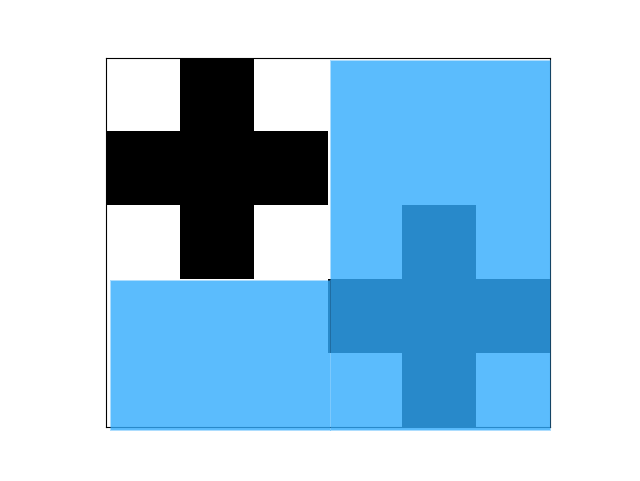
\includegraphics[width=40mm,scale=0.5]{images/convolutional_neural_networks_images/window.png}
            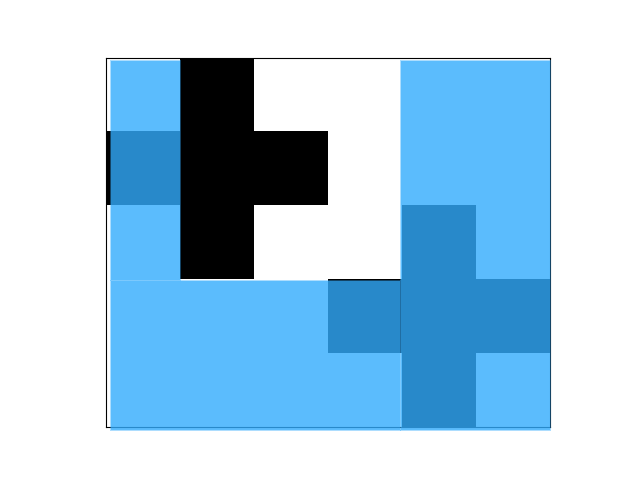
\includegraphics[width=40mm,scale=0.5]{images/convolutional_neural_networks_images/window2.png}
            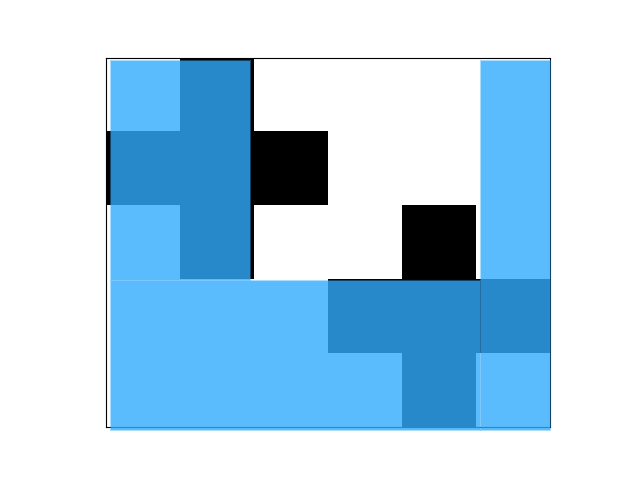
\includegraphics[width=40mm,scale=0.5]{images/convolutional_neural_networks_images/window3.png}
            
            \caption*{In this example, we focus on a 3x3 segment of our data.}
        \end{figure}

        
    \end{itemize}

    This kind of structure is useful for image processing: nearby pixels tend to be related to each other.
        \note{They might form a single line, or a corner, for example.}

    \begin{itemize}
        \item By prioritizing "nearby" information, we can create models that easily find those \textbf{localized} patterns.
        
        \item We called this property \textbf{spatial locality}.\\
    \end{itemize}

    \begin{concept}
        CNNs are designed to represent \vocab{locality}:

        \begin{itemize}
            \item In a CNN, \purp{nearby} data is used to search for patterns.
        \end{itemize}

        This allows us to use smaller, \orgg{simpler} models:

        \begin{itemize}
            \item Rather than thinking about every possible connection between data, we only connect "nearby" data. Thus, we need \gren{fewer} parameters.
        \end{itemize}
    \end{concept}




\phantom{}

\subsection{The problem with locality}

    This presents one simple weakness, that we've ignored so far:

    \begin{itemize}
        \item If we focus on information that is \textbf{nearby}, we're missing out on information that's \orgg{far away}.

        \item We need a way to encode "distance" of information, that doesn't ignore the "distant" info.\\
    \end{itemize}

    \begin{concept}
        If information is spread over \vocab{long distances}, our CNN model won't capture it.

        \begin{itemize}
            \item If a pattern is \purp{too big} for our CNN filter, we'll have more trouble finding it.
        \end{itemize}
    \end{concept}

    This can become especially problematic for \textbf{language} processing.

    \miniex Consider the following sentence: 

    \begin{itemize}
        \item \redd{The sweater} that I found in the back of my old closet, which I hadn't opened since we moved into the house several years ago, \redd{still fits me perfectly.}
    \end{itemize}

    \phantom{}

    Note that the beginning and the end of this sentence are linked as a single idea: "\blu{The sweater still fits me perfectly}".

    \begin{itemize}
        \item But there's a \purp{huge gap} between these phrases: it might be difficult to connect information over such a wide gap, while \orgg{ignoring} what's in-between. 

        \item This also comes up in longer passages: in a paragraph, the first sentence might create \gren{context} for the last sentence.\\
           
    \end{itemize}

    \begin{concept}
        In language, words can be \purp{far apart}, while still providing important \gren{context} for the meaning of the text.

        \begin{itemize}
            \item Thus, language processing is difficult for models which focus too much on \vocab{locality}.
        \end{itemize}
    \end{concept}

\phantom{}

\subsection{RNNs}

    One useful observation might be that language tends to be \textit{sequential}: words come in a very particular order.\\

    \begin{concept}
        In \vocab{image processing}, we see many pixels at the same time: the whole image is processed in \purp{parallel}.

        In \vocab{language processing}, we hear/read words one-by-one, in order: the data has a \gren{sequential} structure.
    \end{concept}

    Recurrent Neural Networks (RNNs) are, thus, a \textbf{sequential} model, designed for processing language.

    \begin{figure}[H]
        \centering
        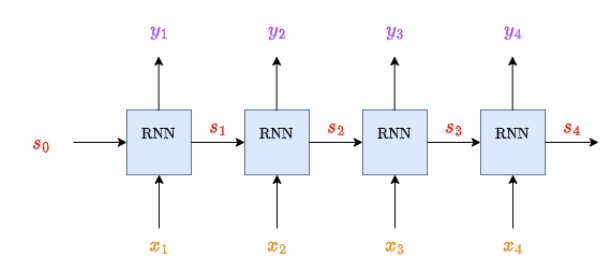
\includegraphics[width=90mm,scale=0.5]{images/transformers_images/rnn_sequential.png}
        \caption*{Each $x_t$ is one word in our sentence: we process the text, one word at a time. After every word, we update our memory ("state" $s_t$). $y_t$ is our output at time $t$.}
    \end{figure}

    By storing information about previous words (using a \gren{state}), our model can "read" each word \purp{in order}, while still remembering earlier parts of the text.

    \begin{itemize}
        \item While a CNN can only observe $k$ consecutive pixels/words in a row, our RNN might be able to contain \textit{some} information about words that are much further back in time.
    \end{itemize}

    How well does this work? RNNs have seen success in the past, but it struggles with \purp{forgetting}: our RNN can only store so much information about words it's seen before.

    \begin{itemize}
        \item As a passage gets longer, our RNN is only paying attention to words it's seen \gren{recently}.
    \end{itemize}

    Moreover, our RNN doesn't have any way to \purp{choose} which words to \orgg{prioritize}: each new word will have to replace some information about older words. 

    \begin{itemize}
        \item So, our RNN naturally prioritizes the most \gren{recent words}.
            \note{The more recent words haven't been replaced yet.}
            
        \item But the most recent word isn't always the most important one, as we saw above (in the sweater example)!\\
    \end{itemize}

    \begin{concept}
        \vocab{RNNs} (Recurrent Neural Networks) tend to struggle with longer bodies of text:

        \begin{itemize}
            \item The \gren{longer} we run our RNN, the less it usually remembers about the \gren{distant} past.
        \end{itemize}

        Moreover, it prioritizes recent words, even when more distant words may be \orgg{more important}.
        
    \end{concept}

    In the end, RNNs have, in most language applications, been replaced by transformers: a different model for language processing.
        \note{However, some transformer models have begun using the concepts of LSTMs, an RNN variant. We won't cover this topic here.}

    

\phantom{}

\subsection{Transformers}

    One clever way to think about this problem is to recognize that our goal is to decide which words are \purp{related} to each other, whether they're nearby or far apart.

    \begin{itemize}
        \item In other words, which words should we pay \orgg{attention} to, in order to understand the text we're reading?
    \end{itemize}

    This is exactly the problem that \vocab{transformer models} solve, using the appropriately named \gren{attention mechanism}.\\

    \begin{clarification}
        In this chapter, we'll use \vocab{transformers} to \purp{process language}, using the mechanism of \orgg{attention}.

        
        \begin{itemize}
            \item But the same tools can be applied to \gren{many other problems}: image and audio processing, robotics, etc.
        \end{itemize}
    \end{clarification}

    


    We'll develop this model in several steps:

    \begin{itemize}
        \item First (11.1), we'll convert words into vectors. One-hot encoding is too simple, so we'll use a different approach: \gren{vector embeddings}.

        \item Next (11.2), we'll figure out which words in a passage are \purp{relevant}(or connected) to each other, using a clever system called \orgg{attention}.

        \item Finally (11.3), we'll put together these ideas to create a complete model, known as a \vocab{transformer}.
    \end{itemize}






\pagebreak
\section{Vector embeddings and tokens}

    \subsection{One-hot encoding isn't enough}

        First, we want to turn words into something computable, like a \gren{vector}.
            \note{It's difficult to try to do math on the word "cheddar". It's not numerical.}
    
        The simplest approach would be \vocab{one-hot encoding}.
            
        \begin{itemize}
            \item \miniex Suppose that we want to classify \textbf{furniture} as table, bed, couch, or chair.
        \end{itemize}
        
        \begin{equation}
            \begin{bmatrix}
              \text{table} \\ \text{bed} \\ \text{couch} \\ \text{chair} 
            \end{bmatrix}
        \end{equation}

        \begin{itemize}
            \item For each class:
        \end{itemize}
        
        
        \begin{equation}
            v_{chair} = 
            \begin{bmatrix}
              0\\0\\0\\ \red{1}
            \end{bmatrix}
            \qquad
            v_{table} = 
            \begin{bmatrix}
              \red{1}\\0\\0\\0
            \end{bmatrix}
            \qquad
            v_{couch} = 
            \begin{bmatrix}
              0\\0\\\red{1}\\0
            \end{bmatrix}
            \qquad
            v_{bed} = 
            \begin{bmatrix}
              0\\\red{1}\\0\\0
            \end{bmatrix}
        \end{equation}

        This approach is simple, but often, it's \textit{too} simple.\\

        \begin{concept}
            \vocab{One-hot encoding} loses a lot of information about the objects it's representing.

            \begin{itemize}
                \item It's hard to say which words are "\gren{similar}" to each other, for example.
            \end{itemize}
        \end{concept}

        \miniex You probably associate the word "\blu{sugar}" with "\blu{sweet}", and "\red{salt}" with "\red{savory}".

        \begin{itemize}
            \item But, if you use one-hot encoding, all of these words are "equally different".
                \note{You could \purp{shuffle} the rows of one-hot vectors, and represent the same information.
                
                \phantom{}
                
                So, we can't use the order of 1's and 0's to determine "closeness": the order can be \gren{freely changed}.}
        \end{itemize}

        \begin{equation}
            v_{salt} = 
            \begin{bmatrix}
              0\\0\\0\\ \red{1}
            \end{bmatrix}
            \qquad
            v_{savory} = 
            \begin{bmatrix}
              \red{1}\\0\\0\\0
            \end{bmatrix}
            \qquad
            v_{sugar} = 
            \begin{bmatrix}
              0\\0\\\red{1}\\0
            \end{bmatrix}
            \qquad
            v_{sweet} = 
            \begin{bmatrix}
              0\\\red{1}\\0\\0
            \end{bmatrix}
        \end{equation}

        In order to incorporate this information, we'll need a better way to represent words as vectors.

    \phantom{}

    \subsection{Word Embeddings: Similarity between words}

        Our new approach will convert each word $w$ into a \purp{vector $v_w$} of \gren{length $d$}.
            \note{Unlike one-hot encoding, we don't require that $d$ equals the size of our vocabulary.}

        \begin{equation}
            w \longrightarrow \pur{v_w} \qquad \qquad \pur{v_w} \in \grn{\RR^d}
        \end{equation}

        \textit{How} do we want to convert words into vectors? Above, we mentioned that one-hot doesn't tell us how \gren{similar} two words are.\\

        \begin{clarification}
            There are many ways for words to be \gren{similar}: similar word length, similar choice of letters, etc.

            But in our case, we're interested in \vocab{semantics}: the \purp{meanings} of the words. We want to know which words have similar meanings.
        \end{clarification}

        \begin{itemize}
            \item \miniex We don't consider "sugar" and "sweet" to be similar because they both start with "s". 
            
            \begin{itemize}
                \item They're similar because of \orgg{meaning}: sugar tastes sweet. Sweet strawberries contain sugar.\\
            \end{itemize}
        \end{itemize}

        \begin{concept}
            We often want our \vocab{word embeddings} $v_w$ to tell us which words are \gren{semantically similar} to each other: which words have similar \purp{meanings}.
            \begin{equation*}
                \text{$v_a$ and $v_b$ are \orgg{similar vectors}} 
                \;\;\iff\;\; 
                \text{$a$ and $b$ are \gren{semantically similar words}}
            \end{equation*}
        \end{concept}

        Our goal is to make this statement true. But we have a problem: these are \textit{concepts}, rather than computable \textit{numbers}. 

        \begin{itemize}
            \item So, we'll have to turn each side into something computable.
        \end{itemize}



    \phantom{}

    \subsection{Vector Similarity: Dot Products}

        First, we'll handle the left side: how do we know if vectors are \gren{similar}? 
        
        \begin{itemize}
            \item We've come across this problem multiple times, and we'll solve it the same way as always: using the \purp{dot product}.\\
        \end{itemize}

        \begin{concept}
            \textit{Review from the Classification chapter}
            
            You can use the \gren{dot product} between vectors $u$ and $v$, \purp{normalized by their magnitudes}, to measure their "\vocab{cosine similarity}". 

            \begin{equation*}
                S_C(u,v) = \frac{u \cdot v}{\abs{u} \cdot \abs{v}}
            \end{equation*}
            
            If two vectors are more \gren{similar}, they have a \gren{larger} normalized dot product. 

            \begin{itemize}
                \item This function ranges from -1 (opposite vectors) to +1 (identical vectors). Perpendicular vectors receive a 0.
            \end{itemize}
        \end{concept}

            \note{We call it "cosine similarity", because this is equal to the cosine of the angle $\alpha$ between $u$ and $v$.}

        \begin{figure}[H]
            \centering
            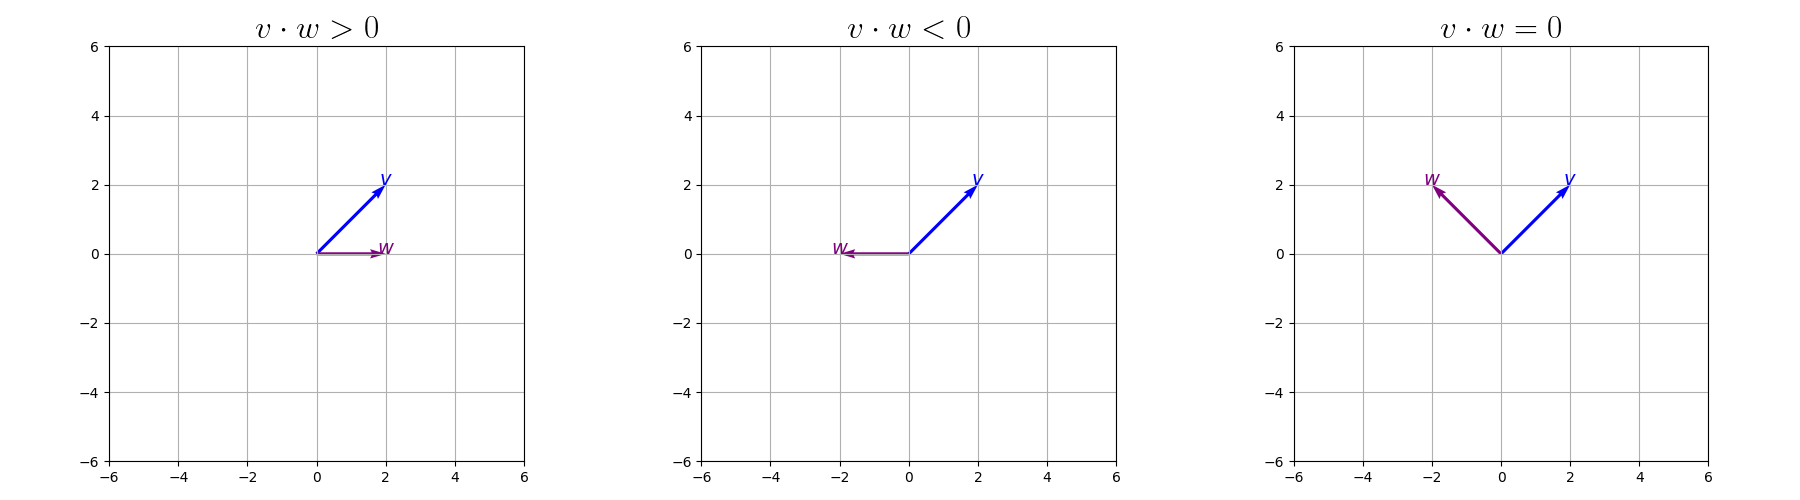
\includegraphics[width=140mm,scale=0.5]{images/transformers_images/dot_product_demo.png}
            
            
            \caption*{We can see here what we mean by "similar" or "dissimilar".}
        \end{figure}

        \begin{clarification}
            You can use $S_C(u,v)$ to measure the \gren{similarity} between two vectors, ignoring magnitude.

            But for simplicity, we'll skip the \purp{normalizing} step, and just take the \vocab{dot product}:

            \begin{equation*}
                S_D(u,v) = u \cdot v = u^\top v
            \end{equation*}
        \end{clarification}

        

        We're getting closer to a computable form:

        \begin{equation}
            \overbrace{ 
                (v_a \cdot v_b) \text{ is \orgg{large}}
            }^{\text{ \lblu{Similar vectors}}}
            \;\;\iff\;\; 
            \text{$a$ and $b$ are \gren{semantically similar words}}
        \end{equation}

    \pagebreak

    \subsection{Word2vec}

        Next, we should get into the math of how to determine which words are likely to be \gren{similar}.

        \begin{itemize}
            \item But this is a bit cumbersome, and isn't really necessary for understanding transformers.
                \note{The short version: we expect words which frequently appear in the same contexts, to be similar.}
        \end{itemize}

        So, we relegate this mathematical labor to Appendix D, where we'll get into the details of \vocab{skipgram} and \vocab{word2vec}.\\

        \begin{definition}
            We can think of \vocab{word2vec} as a system for \orgg{word embeddings} where words which have \gren{similar meanings}, have \purp{similar vector embeddings}.

            \begin{itemize}
                \item Most commonly, we measure "vector similarity" with the \vocab{dot product}.
            \end{itemize}
        \end{definition}

        Instead, we'll skip a couple steps, and look at things from a high level.

    \phantom{}

    \subsection{Probability}

        Our goal is to be able to numerically talk about the "similarity" or "relatedness" of words. 

        Above, we represent this with a \purp{dot product}: this gives us a \orgg{real number} $u \cdot v \in \RR$.
        
        \begin{itemize}

            \item This number isn't very \gren{meaningful}, though. For example, what does a "similarity of 37" even mean? Is that high? Is that low?
        \end{itemize}

        \phantom{}

        Generally, our best bet for understanding a number like this is to \orgg{compare} it to other numbers.
            \note{You know that someone who is 6'5" is really tall, because you know how tall other people tend to be.}

        So, let's think about the \purp{relative} similarity of words: if we have two words, $w_1$ and $w_2$, which one is $v$ \gren{more related} to?

        We'll focus on one simple tool for comparison: \vocab{probability}. 

        \begin{itemize}
            \item One way to think about it is, "how likely is $w_i$ to be the \gren{most relevant} word to $v$, in any given context?"
                \note{In skipgram, our probability comes from asking, "how likely is $w_i$ to show up in the same context?"}

            \item Alternatively, "how \purp{confident} are we that these words are actually closely related, compared to others?"
        \end{itemize}

        \phantom{}

        The \textbf{higher} the probability of word $w_1$, the \textbf{lower} the probability of word $w_2$, and vice versa.

        We'll represent this "relatedness of word $w_i$ to word $v$" as probability $P\big(w_i \mid v\big)$.\\

        \begin{concept}
            One way to describe the \gren{relatedness} of different words $w_i$ is with a \purp{probability} \phantom{fillertext} $P(w_i \mid v) $.

            This has a few advantages:

            \begin{itemize}
                \item A probability is easier to \orgg{interpret} than a real number.

                \item We can directly \gren{compare} different words.

                \item We can systematically \purp{convert} our dot product to a probability.
            \end{itemize}
        \end{concept}

            \note{This "probability" interpretation is a bit better justified if you read the skipgram section.}

        How do we turn a \gren{real number} $v_a \cdot v_b$ into a \purp{probability} $P\big(b \mid a\big)$? 

        \begin{itemize}
            \item For a probability, we need to compare $b$ to every other word: this is a \orgg{multi-class problem}, using the \vocab{softmax function}.
        \end{itemize}

        \begin{equation}
            \operatorname{Softmax}(z_k) = \frac{e^{z_k}}{ \sum_i e^{z_i}}
        \end{equation}

        Let's review the concept behind "softmax":\\

        \begin{definition}
            Suppose that we have \purp{$n$ possible words} ($n$ "classes"), and we want to figure out which one is \gren{correct}.
            
            The \vocab{$\nth{k}$ class} has a score, \org{$z_k$}, used to compute probability.

            \begin{itemize}
                \item The bigger $z_k$ is, the \purp{more likely} $k$ is to be the \gren{correct class}.
            \end{itemize}

            \phantom{}

            To keep it \gren{positive}, $z_k$ is converted to \org{$e^{z_k}$}: each $e^{z_i}$ competes to see which class is more likely.

            \begin{itemize}
                \item To create a probability, we \purp{compare} the score of class $k$ to all of our other classes, using \vocab{softmax}.
            \end{itemize}

            \begin{equation*}
                \overbrace{
                    e^{z_k}}^{\text{\lblu{Class k}}} 
                \text{\; vs \;} 
                \overbrace{ 
                    \sum_i e^{z_i} }^{\text{\lblu{All classes}}}
                \quad \quad \Longrightarrow \quad \quad  \operatorname{Softmax}(z_k) = \frac{e^{z_k}}{ \sum_i e^{z_i}}
            \end{equation*}
            
        \end{definition}

        We repeat this process for every possible word $i$, to get all of our predictions.

        \phantom{}

        What is our "score" $z_k$? We could use $(v_a \cdot v_b)$:

        \begin{itemize}
            \item The higher $(v_a \cdot v_b)$ is, the more \gren{similar/related} we expect $a$ and $b$ to be.

            \item The same is true for $z_k$: if $z_k$ is larger, then our \purp{probability} goes up.
        \end{itemize}

        So, we can use our dot product as a "score" $z_k$:

        \begin{equation}
            z_b = \red{v_a} \cdot \grn{v_b}
        \end{equation}

        We'll plug this into our probability equation:\\

        \begin{kequation}
            The \gren{more similar} (bigger dot product) $a$ and $b$ are, the \purp{more likely} we predict to find them together.

            \begin{itemize}
                \item We use a \vocab{softmax} to compute this probability for each possible word $b$.
            \end{itemize}

            \begin{equation*}
                    \given{ b }{ a } 
                    \quad=\quad
                    \frac{e^{\red{v_a} \cdot \grn{v_b}} }{ \sum_i e^{\red{v_a} \cdot \blu{v_i} }}
            \end{equation*}

            Or, in alternate notation: 
            
            \begin{equation*}
                \given{ \grn{b} }{ \red{a} } 
                \quad=\quad
                \frac{  \phantom{ \Bigg|} 
                \exp \Big(\red{v_a} \cdot \grn{v_b}\Big) }
                {\phantom{ \Bigg|}
                \sum_{\blu{i}} \exp \Big(\red{v_a} \cdot \blu{v_i} \Big) }
            \end{equation*}
        \end{kequation}

        This kind of interpretation makes our word embeddings a bit more \gren{useful}.

        \begin{itemize}
            \item Later, we'll find that it's the most important part of making \purp{transformers} work!
        \end{itemize}




    

         





    

    \pagebreak
    
    \subsection{"Adding" words together}

        Our word2vec system works under the hope that these vector embeddings can accurately represent the \purp{meanings} of words.

        \begin{itemize}
            \item In practice, this assumption works \gren{surprisingly well}, for being so simple.
        \end{itemize}

        One example is the idea of "\orgg{adding}" words together. Normally, it's hard to say how to "add words" together, but we \textit{do} know how to add \purp{vectors}.

        Consider the following example:

        \begin{equation}
            v_{king} - v_{man} + v_{woman}  \quad\approx\quad v_{queen}
        \end{equation}

        This sort of reasoning makes sense to most english speakers: 

        \begin{equation}
            \overbrace{ v_{king} - v_{man} }^{\text{ruler}} \;\;+\;\; v_{woman} 
            \quad\approx\quad \overbrace{v_{queen}}^{\text{female ruler}}
        \end{equation}

        We can repeat this process for other words:
            \note{Paris is the capital of France, and Rome is the capital of Italy.}

        \begin{equation}
            v_{paris} - v_{france} + v_{italy}  \quad\approx\quad v_{rome}
        \end{equation}

        \begin{concept}
            Transforming a word into a \orgg{vector} allows you to use vector operations, like \gren{addition} and \purp{subtraction}.

            \begin{itemize}
                \item The result can be surprisingly \gren{meaningful}, for some word combinations.
            \end{itemize}

            This approach doesn't always work, but the fact that it works \textit{sometimes} suggests that our vectors might capture real information about the "\purp{meanings}" of words.
        \end{concept}

        That said, this approach is often an over-simplification:\\

        \begin{concept}
            Reducing a word to a \purp{single vector} can cause problems, because the same word might change its meaning, based on \gren{context}.
        \end{concept}

        \begin{itemize}
            \item \miniex For example, the word "bank" has a very different meaning when you compare "bank account" to "river bank".
        \end{itemize}

        This idea of "context" is what we hope to solve next.

    \pagebreak



    \subsection{Tokenization}

        One clarification, before we move on: so far, we've talked about predicting whole \gren{words}, because it's easy to work with.

        \begin{itemize}
            \item But often, for language analysis, we break up words into parts, called \vocab{tokens}.

            \item These are the objects we study/predict, rather than whole words.\\
        \end{itemize}

        \begin{definition}
            Rather than using/predicting entire \orgg{words}, we use \purp{small parts of words}, called \vocab{tokens}.

            \begin{itemize}
                \item A "token" is the \gren{smallest unit} in our language model.
            \end{itemize}
        \end{definition}

        \begin{itemize}
            \item \miniex You might break up the word "eating" into "eat" and "ing": both are meaningful, by themselves.

            \item This process of turning words into tokens is called \vocab{tokenization}.
        \end{itemize}

        While "tokens" are used more often than "words", words often make for better examples, so we'll keep using them through the rest of this chapter.\\

        \begin{clarification}
            We'll continue using words (instead of tokens) for examples, when it's convenient.
        \end{clarification}

    

\pagebreak
    
\section{Attention}

    Our \orgg{word embedding} technique has given us a basic way to talk about which words are "\gren{related}".

    \begin{itemize}
        \item We can even use this to learn some about the "\purp{meanings}" of words.
    \end{itemize}

    But there's some work to be done:\\

    \begin{concept}
        Our \vocab{word embedding} technique has two major problems, for representing the \purp{meanings} of words:

        \begin{itemize}
            \item There's a lot of information we're \purp{missing}: \gren{similarity} to other words isn't enough. We'll need a vector to represent that information.
    
            \item The meaning of a word is \orgg{contextual}: the sentence you put a word in, will affect its meaning.
        \end{itemize}
    \end{concept}

    

    It may not look like it, but our \purp{word embedding} technique has already given us the basic tools we need to solve these problems.

    Here's the basic idea, for how we handle each problem:\\

    \begin{concept}
        We'll create a system that solves both of these problems, using \purp{3 word embeddings}: \org{$v$}, \org{$k$}, and \org{$q$}.

        \phantom{}

        \begin{itemize}
            \item We'll \orgg{embed} \gren{information} about each word in a \vocab{value vector} $v$.
    
            \item When finding the \purp{meaning} of a word, we'll calculate \gren{context} from nearby words.
    
            \begin{itemize}
                \item We'll use \gren{word similarity} to figure out which parts of the context are \purp{most important}.
                
                \item For this purpose, word will need \orgg{two embeddings}: a \vocab{key vector} $k$, and a \vocab{query vector} $q$.
            \end{itemize}
        \end{itemize}

        \phantom{}

        The result is a powerful model called the \vocab{attention mechanism}.
    \end{concept}

    This description is over-simplified, which is why we'll need to go into detail below.

    

    




    \phantom{}

    \subsection{The Attention Mechanism: queries, keys}

        Let's consider an \purp{example}, to get used to the idea of $k$, $v$, and $q$.

        Suppose we want a general idea of what "mexican" food is like. We'll need to consider lots of foods, and take an \gren{average} of those we consider to be "mexican".
            \note{Admittedly, we're turning "mexican-ness" into a number, which can be a bit strange. 
            
            \phantom{}
            
            It may help to think this way: "if someone is talking about mexican food, how often are they talking about this food?"}

        \phantom{}

        This problem comes in three parts: let's consider the first two, "query" and "key".

        \begin{itemize}
            \item \vocab{Query $q$}: we're searching for "mexican" food. The word "mexican" is represented by a \purp{query vector} $q$. 
            
            \begin{itemize}
                \item This is like our previous \orgg{word2vec} embedding: if two vectors are similar, then we expect them to have similar/related \orgg{meanings}.
                \item So, we'll \gren{compare} $q$ to each food, to see which foods are 'close' to mexican.\\
            \end{itemize}

            \begin{definition}
                The \vocab{query vector} $q$ represents a word, that we're \gren{comparing} to \purp{several other words} ("keys").

                \begin{itemize}
                    \item It answers the question, "what kinds of words are we \orgg{searching} for?" 
                \end{itemize}

                Using word embeddings, we design $q$ to be "meaningful": similar words, should have similar vectors.
                
                \begin{itemize}
                    \item And we expect \purp{similar words} to be \gren{more relevant} to our query.
                \end{itemize} 
            \end{definition}

            \phantom{}

            \item \vocab{Key $k$}: Each food (apple, burrito, sushi...) has a \purp{key vector} $k$, representing it. 
            
            \begin{itemize}
                \item A \orgg{word2vec}-style embedding, just like the \orgg{query}.

                \item Combining $k$ and $q$ will tell us which foods are \gren{'more' mexican}.\\

            \end{itemize}

            \begin{definition}
                The \vocab{key vector} $k$ represents a word, that we want to \gren{compare} to \purp{the query} $q$.

                \begin{itemize}
                    \item It answers the question, "what kinds of searches does this word \orgg{match}"?
                \end{itemize}

                Because it's a word embedding, which encodes meaning, we expect that, if \purp{$k$ and $q$ are similar}, then our key word is \gren{more relevant} to our query.
            \end{definition}
        \end{itemize}

        Each embedding has a role: a \purp{query} is used to search for relevant words, and a \gren{key} is responding to that search, on behalf of one word.
            \note{Reminder that when we say "word", we're simplifying: we could talk about any kind of token.}

        \begin{concept}
            Another way we could view keys vs. queries:

            \begin{itemize}
                \item \orgg{Query vector $q$}: asks, "how relevant are these words/tokens \purp{to me}?"

                \item \orgg{Key vector $k$}: asks, "how relevant is my word \gren{to the query}?"
            \end{itemize}
        \end{concept}


        Notice that we've made a perspective shift, in how we view word embeddings:\\

        \begin{concept}
            When we were developing word2vec, we wanted \purp{similar vectors} to represent \gren{semantically similar} words.

            \begin{itemize}
                \item But, in this case, we're less focused on "similarity", than \orgg{relevance}.
            \end{itemize}

            We look for \purp{keys} that are the \orgg{most relevant} to our \gren{query}.

        \end{concept}

        These two ideas don't necessarily conflict, but they have somewhat different goals.

    \phantom{}

    \subsection{The Attention Mechanism: attention weights}

        How do we compute how similar $k$ and $q$ are? The same way as we did for word2vec: we use a \gren{dot product}.\\

        \begin{kequation}
            We can get a score for how \gren{relevant} the word $b$ is to word $a$, by taking the \purp{dot product} between \orgg{$b$'s key}, and \orgg{$a$'s query}.

            \begin{equation*}
                q_a \cdot k_b  
            \end{equation*}

            We can also write this as matrix multiplication:

            \begin{equation*}
                q \cdot k = q^Tk
            \end{equation*}
        \end{kequation}

        This gives us a "\orgg{score}": the higher $k \cdot q$ is, the more similar they are.

        \begin{figure}[H]
            \centering
            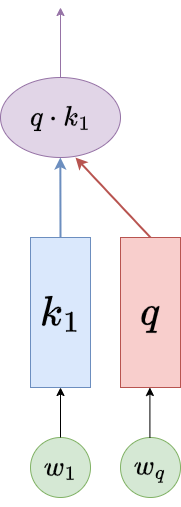
\includegraphics[width=0.1\linewidth]{images/transformers_images/k_dot_q.png}
            \caption*{We convert $w_1$ and $w_q$ into a key and query, respectively, before taking the dot product.}
        \end{figure}

        \begin{notation}
            Note that $k$ and $q$ have to have the \vocab{same length}: they're both $(d_k \times 1)$ column vectors.
        \end{notation}

            \note{If their lengths don't mach, we can't take the dot product.}

        But we're not just considering one key word: we're considering \gren{all of of them}.

        \begin{itemize}
            \item In our "mexican food" example, we need to check every food, to see which ones best fit the category.
        \end{itemize}

        \begin{figure}[H]
            \centering
            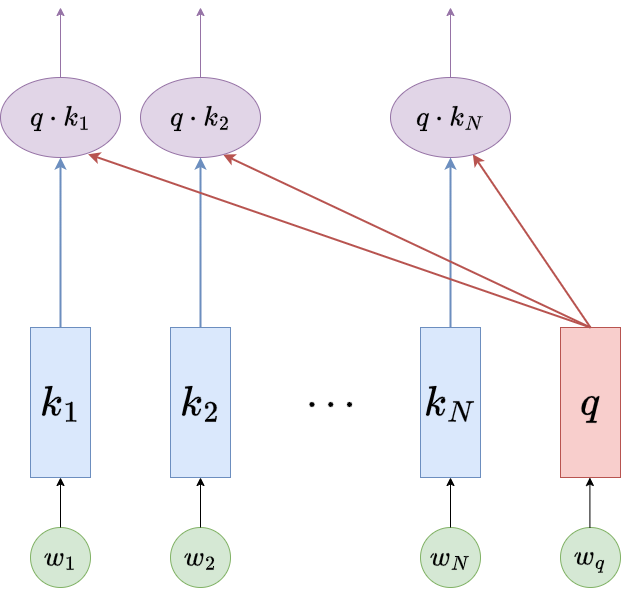
\includegraphics[width=0.3\linewidth]{images/transformers_images/k_dot_q_all.png}
            \caption*{We re-use our query $q$ for every single dot product.}
        \end{figure}

        \begin{notation}
            We have $N$ distinct keys.
        \end{notation}

            \note{In the official notes, we use $n$ instead of $N$. This doesn't affect any of our math.}

        How do we compare each of these keys?

        \begin{itemize}
            \item Once again, we'll reuse a tool from word2vec: \vocab{softmax}.\\
        \end{itemize}
        

        \begin{kequation}
            We can compute the relative \orgg{relevance} of a key $k_j$, by:

            \begin{itemize}
                \item \gren{Comparing} each key $k_i$ to $q$ ($q \cdot k_i$)

                \item Use \purp{softmax} to compute $p(k_j|q)$: given query $q$, how important is $k_j$?
            \end{itemize}


            \begin{equation*}
                    \given{ \grn{k_j} }{ \red{q} } 
                    \quad=\quad
                    \frac{ \phantom{\Big|}  e^{\red{q} \cdot \grn{k_j}} \phantom{\Big|}}
                    {\phantom{\Big|} \sum_i e^{\red{q} \cdot \pur{k_i} } \phantom{\Big|}}
            \end{equation*}

            $\given{ \grn{k_j} }{ \red{q} }$ tells you, "how much \orgg{attention} should $q$ pay to $k_j$"? 

            \begin{itemize}
                \item Thus, we call $\given{ \grn{k_j} }{ \red{q} }$ an \vocab{attention weight}.
            \end{itemize}
        \end{kequation}

        \begin{figure}[H]
            \centering
            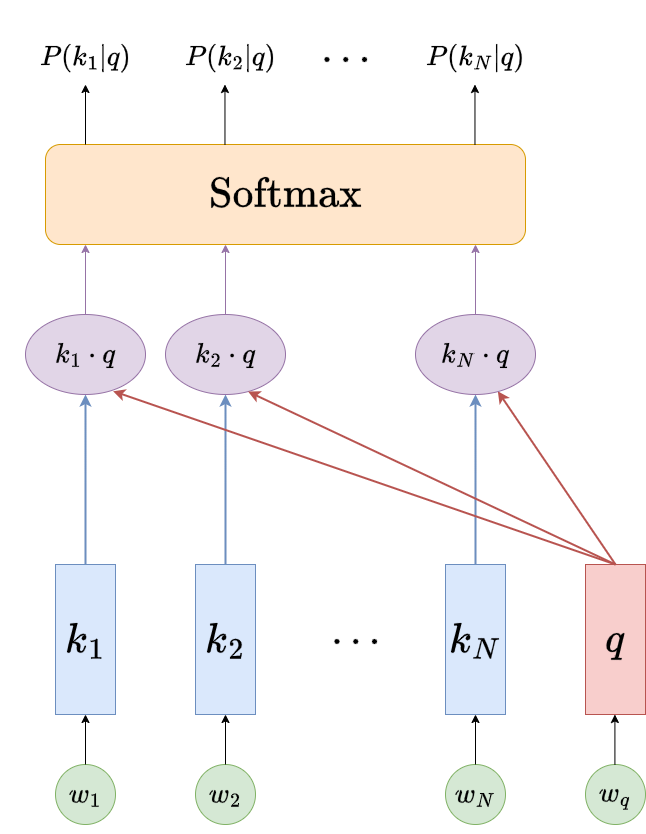
\includegraphics[width=0.3\linewidth]{images/transformers_images/softmax_attention.png}
            \caption*{Finally, we've converted each word into their "probability" of being relevant.}
        \end{figure}

        One notational thing: we can write this a bit more densely.

        \begin{itemize}
            \item So far, we've been computing $q^Tk_i$ for each $k_i$ term \gren{separately}.

            \item But, one benefit of matrix multiplication, is that we can \purp{combine multiple operations} into one.
        \end{itemize}

        First, we'll \gren{combine} all of our key vectors into a matrix $K$:
            \note{This matrix has shape $(N \times d_k)$: the transpose of what you might expect.}

        \begin{equation}
            K = 
            \begin{bmatrix}
                \vertbar & \vertbar  & \     & \vertbar \\
                k_1 & k_2 & \ldots & k_N \\
                \vertbar & \vertbar  &        & \vertbar
            \end{bmatrix}^\top
        \end{equation}

        With that, we can compute all of our dot products \purp{at the same time}:
            \note{This product has shape $(1 \times N)$.}

        \begin{equation}
            q^\top K^T = 
            \begin{bmatrix}
                q \cdot k_1   \\ q \cdot k_2  \\ \vdots \\ q \cdot k_N  \\
            \end{bmatrix}^\top
        \end{equation}

        And we can combine all of these together into a softmax.\\

        \begin{kequation}
            By combining all of our keys into a matrix $K$, we can compute all of our \vocab{attention weights} \gren{at the same time}.

            \begin{equation*}
                \given{ \grn{K} }{ \red{q} }  \quad=\quad
                \begin{bmatrix}
                    \phantom{\Big|} 
                    \mathbf{P} \big( \grn{k_1} \;\big|\; \red{q} \big) \phantom{\Big|} \\
                    \phantom{\Big|}
                    \mathbf{P} \big( \grn{k_2} \;\big|\; \red{q} \big) 
                    \phantom{\Big|}\\
                    \vdots \\
                    \phantom{\Big|}
                    \mathbf{P} \big( \grn{k_N} \;\big|\; \red{q} \big) 
                    \phantom{\Big|}\\
                \end{bmatrix}^\top
                \quad=\quad
                \operatorname{softmax} \big( \red{q^\top}\grn{K^\top} \big)
            \end{equation*}

            It has shape $(1 \times N)$.
        \end{kequation}

            \note{Note that here, softmax creates a row vector.}


        \begin{figure}[H]
            \centering
            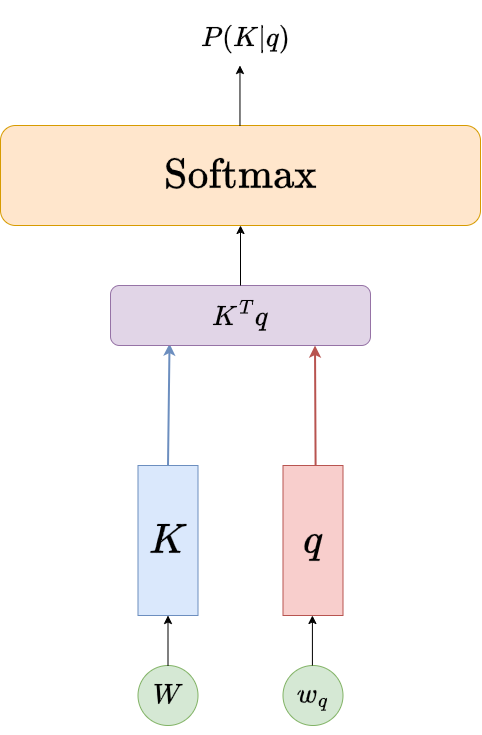
\includegraphics[width=0.3\linewidth]{images/transformers_images/condensed_attention_weights.png}
            \caption*{Now, our diagram is visually simpler, though it reflects the same information. "MatMul" means "Matrix Multiplication".}
        \end{figure}


    \phantom{}

    \subsection{Scaling factor for softmax}

        One pragmatic detail. First, let's quickly define:\\

        \begin{notation}
            Reminder that keys and queries are both vectors of length $(d_k \times 1)$.
        \end{notation}

        We have one problem: the larger $d_k$ is, the more terms in our dot product: our dot product can grow unreasonably \gren{large}.

        \begin{itemize}
            \item This can cause computational issues.
        \end{itemize}

        So, we \purp{normalize} our dot product by a factor of $\sqrt{d_k}$.\\

        \begin{kequation}
            When computing \vocab{attention weights}, we \orgg{normalize} our dot product $q^Tk$ by a factor $\sqrt{d_k}$.

            \begin{itemize}
                \item This compensates for the fact that longer vectors will create larger dot products.
            \end{itemize}

            So, when computing our attention weights $a$, we use the formula:

            $$a(q,K)=\operatorname{softmax} \Big( \frac{ \red{q^\top}\grn{K^\top} }{\sqrt{d_k}} \Big)$$

            It still has shape $(1 \times N)$.
        \end{kequation}

        \begin{figure}[H]
            \centering
            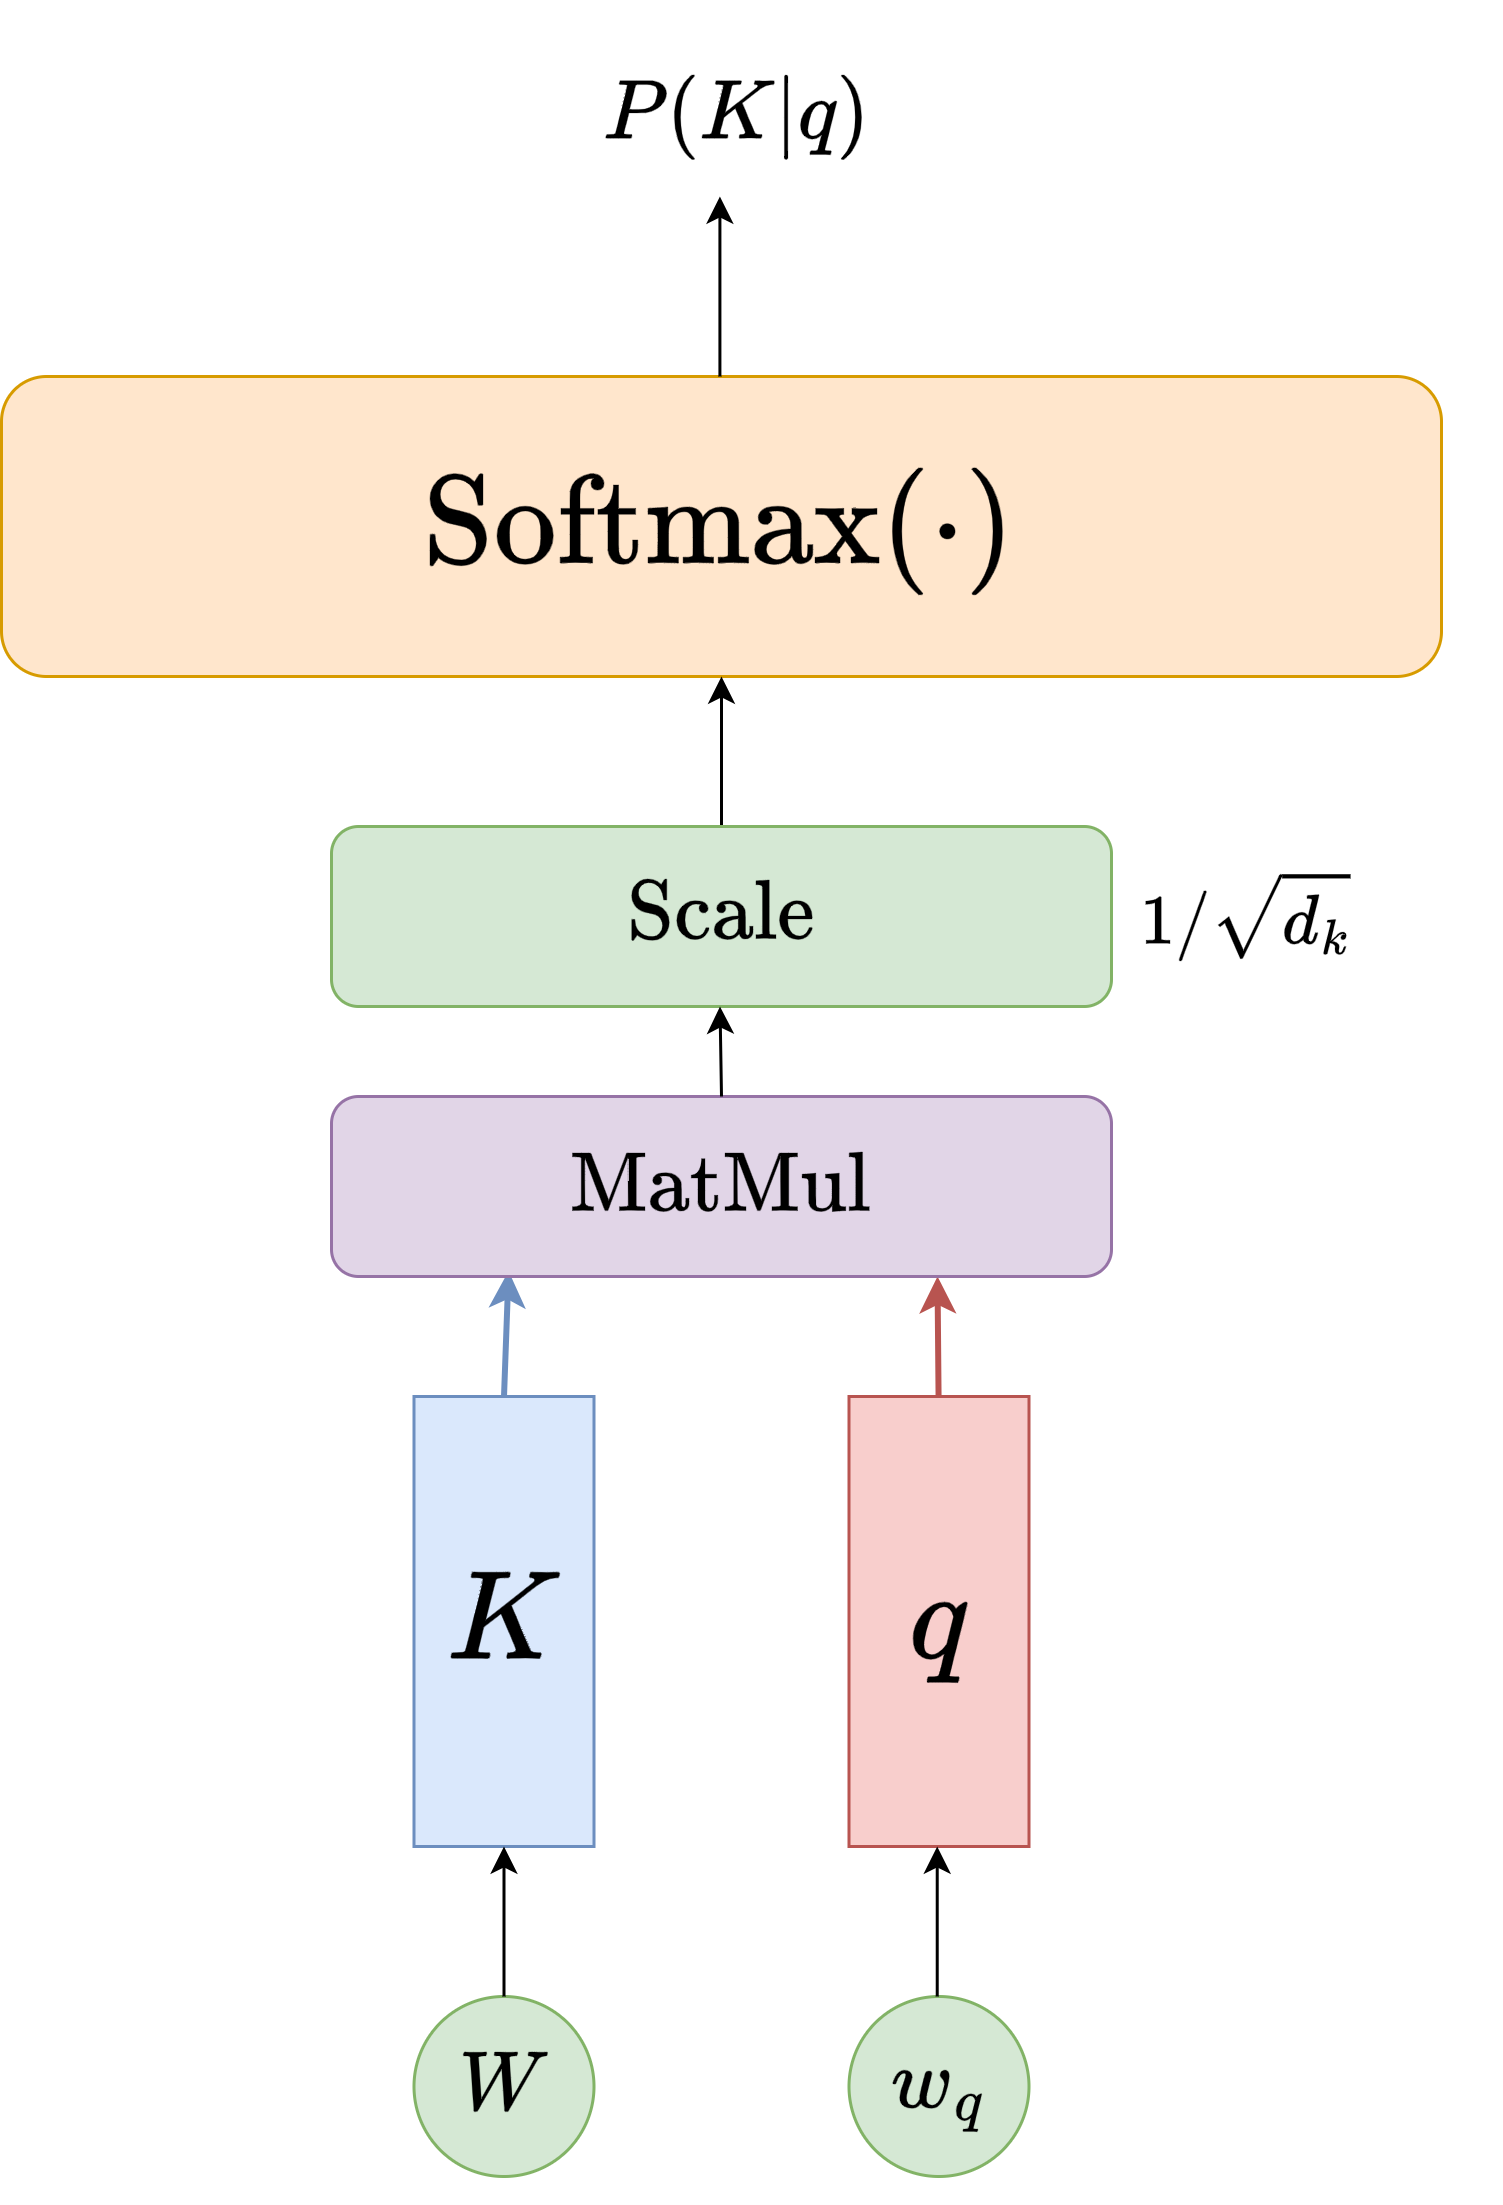
\includegraphics[width=0.3\linewidth]{images/transformers_images/condensed_attention_weights_scaled.png}
            \caption*{We scale down our MatMul by the appropriate factor.}
        \end{figure}

        




    \phantom{}

    \subsection{The Attention Mechanism: values, attention}

        Now, we have a collection of \orgg{attention weights}: each one tells us relevant each word is to $q$.

        \begin{itemize}
            \item Now, we want to make them useful. Our original goal was to get an \gren{average} sense of what "mexican" food is like.
        \end{itemize}

        To make this concrete, we'll introduce our third embedding: the \purp{value vector}.

        \begin{itemize}
            \item \vocab{Value $v$}: Each food has a \purp{value vector}, directly storing information about a word.

            \begin{itemize}
                \item Unlike the key/query vectors, this embedding isn't based on \orgg{similarity} to other words.

                \item Instead, it usually contains more direct \purp{information} about our word: in this example, maybe it contains the price, calories, ingredients, etc.
                    \note{Note that, in a real model, value vectors are often "learned" during training. So, they won't always contain such simple, easily explained data.}\\
            \end{itemize}

            \begin{definition}
                The \vocab{value vector} $v$ represents a word, and stores useful \gren{information} that it can contribute to the \purp{query}.

                \begin{itemize}
                    \item It answers the question, "what useful data could this word contribute to the query?"
                \end{itemize}

                By \gren{adding together} the value vectors from each word \orgg{relevant} to the query, we can get an overall "\purp{averaged value}" for $q$.
            \end{definition}
        \end{itemize}

        \begin{figure}[H]
            \centering
            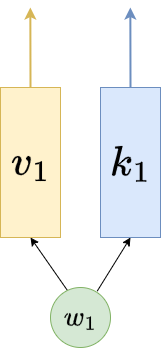
\includegraphics[width=0.1\linewidth]{images/transformers_images/value_key.png}
            \caption*{Each word has both a value and a key attached to it.}
        \end{figure}

        For our example, let's suppose that the value vector contains price, calories, and salt.

        \begin{equation}
            v_i = \begin{bmatrix}
                \text{price}_i \\ \text{cal}_i \\ \text{salt}_i
            \end{bmatrix}
        \end{equation}

        We want to get an "average" calorie count for mexican food.

        \begin{itemize}
            \item Some foods are \gren{common} for mexican food, and some are more rare.

            \item So, to get an average, we'll need to \orgg{emphasize} more "common" mexican food.
        \end{itemize}

        How do we do that? Using our \vocab{attention weights}: the larger the attention weight, the more "\orgg{relevant}" a food is to our mexican food calculation.

        If we use $q$ to represent \red{mexican} food, and $k_i$ is the \gren{key} for the $\nth{i}$ food, we get:

        \begin{equation}
            \text{cal}_{q} = 
            \overbrace{
                \sum_i P(\grn{k_i}|\red{q}) \;\; \text{cal}_{i}
            }^{\text{Weighted average}}
        \end{equation}

        Rather than repeating this process for each row of $v$, we can just do a \vocab{weighted average} of the whole vector, at the same time:

        \begin{equation}
            v_{q} = 
                \sum_i P(\grn{k_i}|\red{q}) \; v_{i}
        \end{equation}

        \begin{kequation}
            Each word $i$ has a \orgg{value vector} $v_i$, which represents all of the useful \gren{information} it can provide to the \purp{query}.

            \begin{itemize}
                \item We can use a \vocab{weighted average} to combine all of these value vectors together: this provides the "\purp{overall context}" for the query.

                \item Each value is weighted based on its \orgg{attention weight} $P(\grn{k_i}|\red{q}) $: how likely it is to be relevant.
            \end{itemize}

            \begin{equation*}
                v_{q} = 
                    \sum_i P(\grn{k_i}|\red{q}) \; v_{i}
            \end{equation*}

            This is the calculation for \vocab{attention}.
        \end{kequation}

        Just like we did for the $k_i \cdot q$ operation, we can re-write this in terms of matrix multiplication.

        \begin{itemize}
            \item We'll change from $P(\grn{k_i}|\red{q})$ to $P(\grn{K}|\red{q})$.
        

            \begin{equation*}
                \given{ \grn{K} }{ \red{q} }  \quad=\quad
                \begin{bmatrix}
                    \phantom{\Big|} 
                    \mathbf{P} \big( \grn{k_1} \;\big|\; \red{q} \big) \phantom{\Big|} \\
                    \phantom{\Big|}
                    \mathbf{P} \big( \grn{k_2} \;\big|\; \red{q} \big) 
                    \phantom{\Big|}\\
                    \vdots \\
                    \phantom{\Big|}
                    \mathbf{P} \big( \grn{k_N} \;\big|\; \red{q} \big) 
                    \phantom{\Big|}\\
                \end{bmatrix}^\top
                \quad=\quad
                \operatorname{softmax}( \red{q^T}\grn{K^T})
            \end{equation*}

            \item We'll stack all of our value functions $v_i$ into a matrix $V$.

            \begin{equation}
                V = 
                \begin{bmatrix}
                    \vertbar & \vertbar  & \     & \vertbar \\
                    v_1 & v_2 & \ldots & v_N \\
                    \vertbar & \vertbar  &        & \vertbar
                \end{bmatrix}^\top
            \end{equation}
        \end{itemize}

        \begin{notation}
            We'll assume that we have $N$ value vectors of length $d_k$.

            \begin{itemize}
                \item $v_i$ has shape $(d_k \times 1)$, $V$ has shape $(N\times d_k )$.
            \end{itemize}
        \end{notation}

            

        Now, we can compute with every value vector at once:
        \note{If you study the classic "\href{https://arxiv.org/pdf/1706.03762.pdf}{Attention is all you need}" paper, you'll find that their version of $k$ and $q$ are transposed compared to ours.}\\

        \begin{kequation}
            We can compute \vocab{attention} using matrix multiplication:

            \begin{equation*}
                \operatorname{Attention} \big( \red{q},\grn{K},\org{V} \big) 
                \quad=\quad 
                \operatorname{softmax} \Big( \frac{ \red{q^\top}\grn{K^\top} }{\sqrt{d_k}} \Big) 
                \org{V} 
            \end{equation*}

            Where $\operatorname{softmax} \Big( \frac{ \red{q^\top}\grn{K^\top} }{\sqrt{d_k}} \Big)$ computes our \purp{attention weights}.

            \begin{itemize}
                \item Under this definition, attention has shape $(1 \times d_k )$.
            \end{itemize}
        \end{kequation}

        \phantom{}

        \begin{definition}
            $\text{Attention}(q,K,V)$ is the \orgg{weighted average} of all of our value vectors (transposed).

            \begin{itemize}
                \item Attention is the \purp{result} of \gren{aggregating} information from $N$ different words: each word is represented by a key $k_i$, and a value vector $v_i$.
            \end{itemize}
        \end{definition}

            

        \begin{figure}[H]
            \centering
            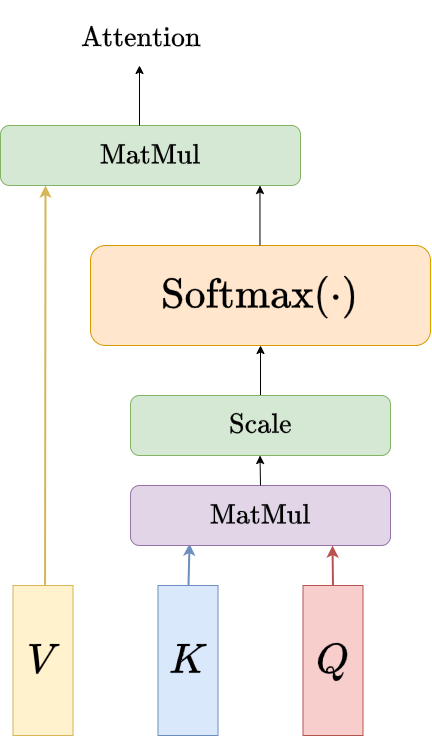
\includegraphics[width=0.3\linewidth]{images/transformers_images/condensed_attention.png}
            \caption*{We now have a completed representation of attention.}
        \end{figure}

        \note{In the "\href{https://arxiv.org/pdf/1706.03762.pdf}{Attention is all you need}" paper, this diagram is analogous to Figure 2 (left).
        
        \phantom{}
        
        Here, we omit the "Mask" layer (discussed later).}

        With this, we can summarize the basic idea of attention:\\

        \begin{concept}
            \vocab{Attention} is a mechanism that allows you to \gren{combine} information from multiple tokens, weighting each token by how \purp{relevant} it is.

            This mechanism is broken into three parts:

            \begin{itemize}
                \item \orgg{Value vector $v$}: \gren{what information} are we trying to combine?

                \item \orgg{Query vector $q$}: what kinds of words are \purp{relevant} to this search?

                \item \orgg{Key vector $k$}: what kinds of searches is this word \gren{relevant} for?
            \end{itemize}

            Each token has a \purp{value vector} (information from that token), and a \gren{key vector} (used to compare this token to the query).
        \end{concept}

        Note that this isn't the \purp{only} way to do attention:\\

        \begin{clarification}
            There are multiple ways we can implement attention.

            \begin{itemize}
                \item For example, we use $q \cdot k$ to measure similarity, but we could \purp{replace} it with a different metric.
            \end{itemize}
        \end{clarification}

            \note{Reminder: a "metric" is just "a way of measuring something. The dot product is a \vocab{similarity metric} for vectors.}

        

        



    \pagebreak

    So far, we've mostly focused on the mathy details of \gren{how} attention works: an abstract idea of "relevance" between words, "combining" the value ("meaning") of different words, etc.

        \begin{itemize}
            \item Here, we'll try something different: we'll focus more on \purp{why} we use attention, and how it applies to a real, concrete situation.
        \end{itemize}

    \phantom{}

    \subsection{Why we need context}

        Attention is designed to integrate information from other, \gren{nearby} words. But why do we need to do this?

        \begin{itemize}
            \item Because language is heavily dependent on \orgg{context}.
        \end{itemize}

        Consider the task of \gren{language translation}: we have a sentence in one language, and we want to convert it into another language, while \purp{preserving the meaning}.

        Let's translate the sentence:

        $$\text{I miss her \red{warm} \blu{smile}.}$$

        We'll focus on the word "warm". 

        \begin{itemize}
            \item Most commonly, "\red{warm}" means "higher-than-average temperature". For example, being under a blanket is warm.

            \item But most humans would say that, in this situation, the word "\red{warm}" means 'friendly' or 'kind'.
        \end{itemize}
        

        We know this because of the \textit{context}: a "warm smile" usually means a "kind smile". The word '\blu{smile}' has \purp{changed the meaning} of the word '\red{warm}'.\\

        

        \begin{concept}
            The meaning of a word can change based on the other words which are \purp{nearby}.

            \begin{itemize}
                \item This is why we need to integrate \vocab{context} for language processing.
            \end{itemize}
        \end{concept}

        If our machine blindly translated "warm", without context, we could've ended up with the wrong meaning in another language.

    \phantom{}


    \subsection{Why we need \textit{attentive} context}

        So, we need to use context. But what makes attention special?

        \begin{itemize}
            \item It allows us to figure out \purp{which words} are most important to us!
        \end{itemize}

        In the above sentence, the word "\blu{smile}" changed the meaning of "\red{warm}".

        \begin{itemize}
            \item How do we know that "\blu{smile}" is the important context word? "\grn{her}" is equally far from "\red{warm}".

            \item Attention handles this for us: we "\vocab{pay more attention}" to the word '\blu{smile}' than the word '\grn{her}', when we're trying to understand "\red{warm}".\\
        \end{itemize}

        \begin{concept}
            \vocab{Attention} allows us to determine which parts of the \orgg{context} are \gren{most important} to a particular word.
        \end{concept}




\pagebreak

    \subsection{Self-attention}
    
        Attention has given us a tool for comparing one word to every other word in a sentence.
    
        \begin{figure}[H]
            \centering
            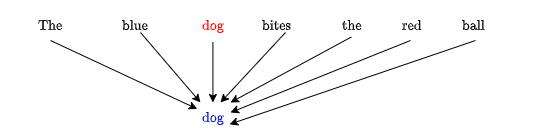
\includegraphics[width=0.6\linewidth]{images/transformers_images/attention_dog.png}
            \caption*{"dog" is represented by a query $q_{dog}$, compared to the key for every other word in the sentence. This gives us our attention weights.
    
            
            Next, we combine these weights with the value vector for each word. This gives us our \vocab{attention}: the "contextual meaning" of the word \redd{dog}. }
        \end{figure}
    
        This has a limitation: we're only focusing on a single word, "dog".
    
        \begin{itemize}
            \item But we need to get the meaning of \purp{every word} in the sentence, based on the context from other words.
        \end{itemize}
    
        \begin{figure}[H]
            \centering
            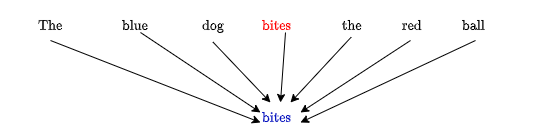
\includegraphics[width=0.6\linewidth]{images/transformers_images/attention_bites.png}
            \caption*{This time, we use the query $q_{bites}$ for the word "bites". However, the key and value vectors are still the same for each word.
            
            We need to repeat this attention process once for each word.}
        \end{figure}
    
        This is interesting: we're seeing how much each word affects each other word in the sentence. We're seeing how the sentence provides context for \orgg{itself}.
    
        \begin{itemize}
            \item This is why we call this \vocab{self-attention}.\\
        \end{itemize}
    
        \begin{definition}
            \vocab{Self-attention} is the process of using attention on every word in a passage.
    
            \begin{itemize}
                \item For the $\nth{i}$ word, we compare it to \purp{every other word} in the passage.
            \end{itemize}
    
            This allows us to interpret each word, based on the \gren{context} provided by the rest of the sentence.
        \end{definition}
    
            \note{Technically, we also compare each word to itself.}
    

    \subsection{Self-attention in matrix form}

        How do we handle this, mathematically?

        \begin{itemize}
            \item When we are getting the attention for word $w_i$, we use its query $q_i$ to compare it to other words in the sentence.
        \end{itemize}

        We've gone from having a single query $q$ to having many $q_i$: one for each word in the sentence.

        \begin{equation}
            Q = 
            \begin{bmatrix}
                \vertbar & \vertbar  & \     & \vertbar \\
                q_1 & q_2 & \ldots & q_N \\
                \vertbar & \vertbar  &        & \vertbar
            \end{bmatrix}^T
        \end{equation}

        Let's note some conventions:\\

        \begin{notation}
            A few useful \vocab{dimensions}: in an attention problem, we have...

            \begin{itemize}
                \item $n_k$ keys of length $d_k$.
                \item $n_q$ queries of length $d_q$.
                \item $n_v$ values of length $d_v$.
            \end{itemize}

            In \gren{practice}, we usually take $d_k=d_q=d_v$, and simply refer to all three as $d_k$.

            \begin{itemize}
                \item Each column vector ($k_i$, $v_i$, $q_i$) has shape $(d_k \times 1)$.
            \end{itemize}

            In \purp{self-attention}, we take $n_k=n_q=n_v$, and simply refer to all three as $N$.

                \begin{itemize}
                    \item Matrices $K$, $V$, and $Q$ all have shape $(N \times d_k)$.
                \end{itemize}
        \end{notation}

        Each of these queries will create a separate set of attention weights, $\text{softmax}(q_i^TK)$.\\

        

        \begin{kequation}
            We define the \vocab{self-attention weight} matrix $A$, to represent all attention weights:

            $$
            A = 
            \begin{bmatrix}
                \text{softmax} \Big( \red{q_1^T} \grn{K^T}/ \sqrt{d_k} \Big) \\
                \text{softmax} \Big( \red{q_2^T} \grn{K^T}/ \sqrt{d_k} \Big) \\
                \vdots \\
                \text{softmax} \Big( \red{q_N^T} \grn{K^T}/ \sqrt{d_k} \Big)
            \end{bmatrix}=
            \text{softmax}\Big(\frac{\red{Q}\grn{K^T}}{\sqrt{d_k}}\Big)$$

            This is an $(N \times N)$ matrix.

            \begin{itemize}
                \item Row $i$ tells us all of the attention weights applied to query $q_i$.
                \item Col $j$ tells us the attention weights for key $k_j$.
                \item Element $\alpha_{ij}$ (row $i$, col $j$) tells us, "how \gren{important} is word $j$ (key) as context for word $i$ (query)"?
            \end{itemize}
        \end{kequation}

            \note{Note that the elements in row $i$ must add up to 1: we have softmax.
            
            \phantom{}
            
            This is not true for column $j$: they're probabilities for different queries.}

        We can use this to get the total attention:\\

        \begin{kequation}
            The \vocab{self-attention} equation is given as 

            $$\text{Attention}(\red{Q},\grn{K},\org{V}) = \pur{A}\org{V} = \text{softmax}\Big(\frac{\red{Q}\grn{K^T}}{\sqrt{d_k}}\Big)\org{V}$$

            It is a $(N \times d_k)$ matrix.
        \end{kequation}

        Row $i$ gives the \purp{averaged value vector} $\ex{y}{i}$ for the $\nth{i}$ word, based on all of the surrounding \orgg{context}. 
            \note{We could view this as the "output" for the $\nth{i}$ word.}

        \begin{itemize}
            \item We can write this in element-wise form:
        \end{itemize}

        $$\ex{y}{i} = \sum_{j=1}^N \alpha_{ij} v_j$$

        One theme we'll run into, many times in this chapter, is that attention-based models benefit from being able to \purp{parallelize}:\\

        \begin{concept}
            \vocab{Transformer Parallelization I}
        
            Computing self-attention can be strongly parallelized:

            \begin{itemize}
                \item Each $q_j^Tk_i$ term is \purp{independent} of the others: we can compute all of the key-query dot products \gren{at the same time}, rather than waiting for one to finish before starting the others.
                \item We can compute each softmax term at the same time, as well.
            \end{itemize}
        \end{concept}

            \note{This remains true if we're using \vocab{cross-attention}, where the keys and queries come from different words.}


\pagebreak

\subsection{Positional Encoding}

    First, a problem we need to address:

    \begin{itemize}
        \item Currently, our key $k_i$ is determined by asking the \purp{identity} of the word at index $i$.

        \item This key doesn't encode information about the \gren{position} of this word in the sentence.
    \end{itemize}

    But clearly, the position of a word will determine its meaning.

    \begin{itemize}
        \item \miniex "The cat lies on the green table" and "the green cat lies on the table" are \redd{not the same}: moving the word "green" to a different index changes its meaning.
    \end{itemize}

    We fix this by adding information to keep track of this position.\\

    \begin{definition}
        We apply \vocab{positional encoding} to each word embedding: each embedding includes information about the \gren{position} of a word in the text.

        \begin{itemize}
            \item This allows our attention mechanism to use this information when deciding the \purp{relevance} of different words.
        \end{itemize}
    \end{definition}

\phantom{}

\subsection{Masking}

    One common use for transformer models is \vocab{text prediction}: learning what word should come next, based on what it has seen so far.

    Typically, we would give our model the text, and give it a chance to try to \purp{predict} each index, \gren{before} it can see it.

    We need to prevent our model from being able to \orgg{cheat}:

    \begin{itemize}
        \item We don't want our model to be able to see the words it's supposed to be predicting.
    \end{itemize}

    \begin{figure}[H]
        \centering
        
\includegraphics[width=0.6\linewidth]{images/transformers_images/masking.png}
        \caption*{So, we'll hide those words, so our model can't see them. In this case, we want our model to predict the next word: "dog".}
    \end{figure}

    This is called \vocab{masking}.\\

    \begin{definition}
        \vocab{Masking} is a technique where we \purp{hide} some information from our model, so it can't use that information.

        \begin{itemize}
            \item For example, if our model is being used to \gren{predict text}, we hide the text that it's trying to predict.
        \end{itemize}

        However, the word "masking" can apply to \textbf{any} situation where we want to hide tokens from the model.
    \end{definition}
    
\pagebreak

\subsection{Attention Heads}

    We have a system for "attention": deciding which words provide the \gren{most important} context/information, and paying more attention to those words.

    But there's something we haven't considered: the "importance" of different words, depends on \purp{what you're interested in}. Let's consider a couple examples:

    \begin{itemize}
        \item \vocab{Syntax}: which words are \gren{subjects, objects, verbs, adjectives}?

        \miniex "The boy kicks the red ball": our focus is on the word "ball". 

            \begin{itemize}
                \item "red" is important for color.

                \item "kicks" is important for knowing what's happening to the ball.

                \item "boy" is important for knowing who is acting on the ball.\\
            \end{itemize}

        \item \vocab{Semantics}: which words change the \gren{meaning} of our target word?

        \miniex "I miss her warm smile": our focus is on the word "warm".

            \begin{itemize}
                \item The word "smile" changes the meaning of warm from 'high temperature' to 'kind'.\\
            \end{itemize}

        \item \vocab{Coreference}: which words are referring to the \gren{same object}?

        \miniex "John said that he isn't hungry": our focus is on the word "John".

            \begin{itemize}
                \item "he" refers to the same object as "John": if we apply something to the word "he", it also applies to "John".\\
            \end{itemize}

    \end{itemize}

    \begin{concept}
        What is "\purp{important}" in a sentence can \gren{change}, based on what you're trying to study.

        \begin{itemize}
            \item And generally, these ideas of "important" won't agree with each other.
        \end{itemize}
    \end{concept}

    Above, we suggested several different perspectives on "what is important".

    \begin{itemize}
        \item Rather than having our attention mechanism try to handle all of these kinds of importance, we could create a \orgg{separate mechanism} for each one of them.
    \end{itemize}

    We'll do just that: each "perspective" will be represented by a different mechanism. We call each of these, \vocab{attention heads}.\\

    \begin{definition}
        A transformer model may use \purp{multiple} attention mechanisms \gren{at the same time}:

        \begin{itemize}
            \item Each attention mechanism is a different "\orgg{perspective}" on our data: it focuses on different aspects of the text (grammar, meaning, tone, etc.)

            \item To accomplish this, each one represents a word $w$ with a different $k$, $q$, and $v$.
        \end{itemize}

        We call each mechanism one \vocab{attention head}.
    \end{definition}

    If we have 3 different attention heads, each one may \purp{encode} the word "silly" differently. We could have three different keys for this one word: $k^1$, $k^2$, and $k^3$.

    \begin{itemize}
        \item Each head will require a distinct word encoding: $\ex{K}{h}$, $\ex{Q}{h}$, and $\ex{V}{h}$.\\
    \end{itemize}

    \begin{concept}
        \vocab{Transformer Parallelization II}
    
        Each attention head uses calculations which are \purp{independent} from the others: we can compute each attention head at the same time!
    \end{concept}

    

    
\pagebreak

\section{Transformers}

    Now that we've built up attention, we'll use it to build a \vocab{transformer}. We'll assume our transformer uses self-attention, though the math works out similarly even if it doesn't.\\

    \begin{definition}
         A \vocab{transformer block} is a collection of attention heads running in \purp{parallel}, applied to the same text.

         A \vocab{transformer} is composed of several transformer blocks in \gren{series}: the output of one block is the input of another.
    \end{definition}


    \subsection{How to create embeddings}

        Something we've ignored for a while is, "how do we construct our \purp{embeddings} $K$, $Q$, and $V$"? 
        
        \begin{itemize}
            \item We aren't actually given them: we're given a sequence of \gren{tokens}: each token is a vector $x$ representing a word. So, our whole body of text is a matrix $X$.
                \note{Each vector is length $d$: this is different from the length of the embedding, $d_k$.}
        \end{itemize}

        We'll compute each embeddings by using a \vocab{linear transformation}:\\

        \begin{kequation}
            We use \vocab{projection matrices} $W_k$, $W_q$, and $W_v$ to transform each \purp{token} $\ex{x}{i}$ into embeddings $k$,$q$, and $v$.

            $$
            \begin{matrix}
                k_i = W_k^\top \ex{x}{i} \\
                q_i = W_q^\top \ex{x}{i} \\ 
                v_i = W_v^\top \ex{x}{i} 
            \end{matrix}$$

            All three projection matrices have shape $(d \times d_k)$. 
        \end{kequation}

            \note{Reminder that:
            
            \phantom{}
            
            $d$ is the original length of $\ex{x}{i}$
            
            \phantom{}
            
            $d_k$ is the length after embedding.}

        All of our tokens are stored in matrix $X$:
            \note{Unlike our usual $X$, this is transposed: shape $(N \times d)$.}

        \begin{equation}
            X = 
            \begin{bmatrix}
                \vertbar & \vertbar  & \     & \vertbar \\
                \ex{x}{1} & \ex{x}{2} & \ldots & \ex{x}{N} \\
                \vertbar & \vertbar  &        & \vertbar
            \end{bmatrix}^T
        \end{equation}

        We can get the keys, queries, and values for all of our vectors in matrix form:\\

        \begin{kequation}
            We can compute $K$, $Q$, and $V$:

            $$
            \begin{matrix}
                K = XW_k \\
                Q = XW_q \\ 
                V = XW_v 
            \end{matrix}$$
        \end{kequation}

        Based on this linear transform, we modify our diagram:

        \begin{figure}[H]
            \centering
            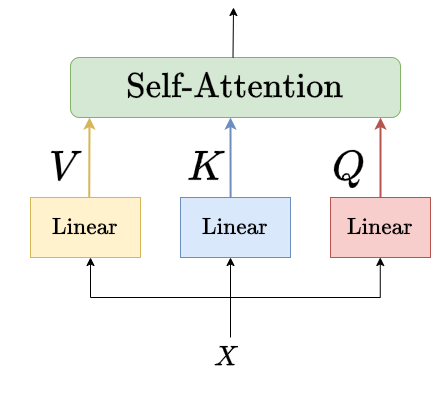
\includegraphics[width=0.3\linewidth]{images/transformers_images/linear_VKQ.png}
            \caption*{We have to generate $V$, $K$, and $Q$ before we can use them.}
        \end{figure}

        \begin{concept}
            One benefit of computing keys, values, and queries based on \vocab{weight matrices} is that we can \gren{train} these matrices: 

            \begin{itemize}
                \item Rather than manually designing the \purp{embeddings}, we can allow our model to learn whichever embedding is most useful.
            \end{itemize}
        \end{concept}

    %These matrices will be trained in the same way as any other weights:

    %\begin{itemize}
    %    \item We include them in a larger model, which we want to train for some task. We use a learning algorithm to optimize the weights, to give better outputs

    %    \item This is it means to "learn whichever embedding is most useful": 
    %\end{itemize}

    \phantom{}

    \subsection{Attention Heads}

        What if we have \purp{multiple} attention heads?\\

        \begin{notation}
            If we have $H$ attention heads in a transformer block we'll indicate the $\nth{h}$ head with:

            $$
            \begin{matrix}
                \ex{K}{h} = XW_{h,k} \\
                \ex{Q}{h} = XW_{h,q} \\ 
                \ex{V}{h} = XW_{h,v} 
            \end{matrix}$$
        \end{notation}

        Each attention head is applied in parallel:

        \begin{figure}[H]
            \centering
            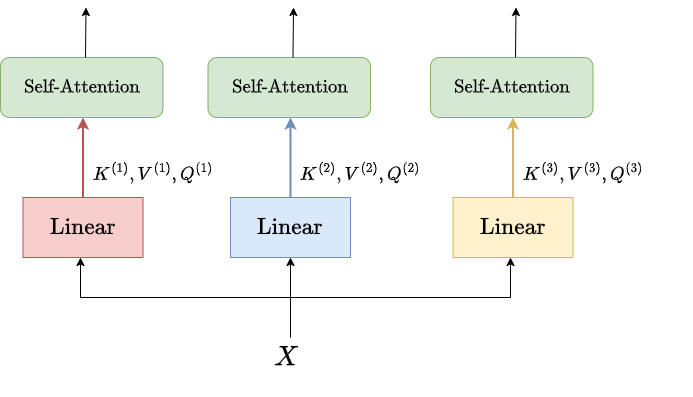
\includegraphics[width=0.5\linewidth]{images/transformers_images/multi_headed_attention.png}
            \caption*{Here's an example with $H=3$ attention heads. Each uses a distinct set of keys, values, and queries.}
        \end{figure}

        To finish off our multi-headed attention unit, we do two more things:

        \begin{itemize}
            \item Transform each token back into the original dimensions: going from length-$d_k$ to length-$d$.
            \item Combine the results from each attention head: we'll do a \gren{weighted average}.\\
        \end{itemize}

        \begin{kequation}
            After computing attention for each head, we take a \orgg{weighted average} of our heads, combining them together:

            \begin{itemize}
                \item For each head, we use matrix $W_{h,c}$ to \gren{scale} the weight of each head, and convert them back to their original \purp{shape}.
                    \begin{itemize}
                        \item $W_{h,c}$ has shape $(d_k, d)$.
                    \end{itemize}
                \item We \gren{add} together the results, gathering information from each head.
            \end{itemize}

            $$u = \sum_{h=1}^{H} \text{Attention}\big(\red{\ex{Q}{h}}, \grn{\ex{K}{h}}, \org{\ex{V}{h}}\big) 
            \;\bro{W_{h,c}}$$ 

            $u$, the final output of our \vocab{multi-headed attention}, has shape $(N \times d)$, where the $\nth{j}$ column represents the $\nth{j}$ token.
        \end{kequation}

        

        \begin{figure}[H]
            \centering
            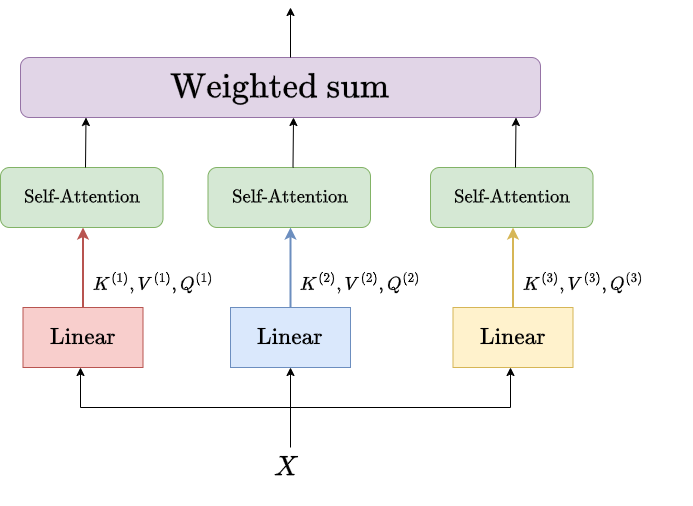
\includegraphics[width=0.5\linewidth]{images/transformers_images/multi_headed_attention_complete.png}
            \caption*{We have our completed multi-headed attention unit!}
        \end{figure}

        \note{In the "\href{https://arxiv.org/pdf/1706.03762.pdf}{Attention is all you need}" paper, this diagram is analogous to Figure 2 (right).
        
        \phantom{}
        
        Instead of directly doing a weighted sum, they concatenate each attention head, and then apply a linear weight $W^o$. 
        
        \phantom{}
        
        These are equivalent.}

        \vspace{150pt}

        Note that this is the same shape as our original input, $X$:

        \begin{equation}
            U= 
            \begin{bmatrix}
                \vertbar & \vertbar  & \     & \vertbar \\
                \ex{u}{1} & \ex{u}{2} & \ldots & \ex{u}{N} \\
                \vertbar & \vertbar  &        & \vertbar
            \end{bmatrix}^\top
        \end{equation}

        In fact, we can compute this multi-headed attention, one $\ex{u}{i}$ at a time.
            \note{Reminder that $\pur{\alpha_{ij}}$ is an attention weight from $\pur{A}$, and $\org{\ex{v}{j}}$ is a value vector of $\org{V}$.}\\

        \begin{kequation}
            We can combine our multi-attention heads as

            $$\ex{u}{i} = \overbrace{\sum_{h=1}^H \bro{W_{h,c}^\top}}^{\text{Heads}} \quad
            \overbrace{\Big( \sum_{j=1}^N \pur{\ex{\alpha_{ij}}{h}} \org{\ex{v_j}{h}} \Big)}^{\text{Attention}}$$
        \end{kequation} 
        
            \note{This is a nested sum: 
            \phantom{}
            
            $\sum_{h,j}(\cdot)$, 

            \phantom{}
            
            not a product of two sums, 

            \phantom{}
            
            $(\sum_h(\cdot)) \cdot (\sum_j (\cdot))$}

    \pagebreak
    

    \subsection{Residual Connections}

    
        Our next component will handle a problem with \purp{deep} neural nets that we've addressed before: vanishing/exploding gradient.\\

        \begin{definition}
            \textit{(Review from Neural Networks 2)}
            
            \vocab{Vanishing gradient} occurs when a deep neural network ends up with \purp{very small gradients} in the \gren{earlier} layers. 
            
            This happens because a deeper neural network has a \gren{longer chain rule}: if all of the terms are \purp{less than one}, they'll multiply into a very small value, "\vocab{vanishing}".
            
            This means that our gradient descent will have \purp{almost no effect} on these earlier weights, \gren{slowing down} our algorithm considerably.
        \end{definition}

        In short: the "further away" from our input layer, the messier our gradients get.

        One simple solution is to include our original, \gren{unmodified} input, deeper in the neural network: we just \purp{add} it, so that our second layer gets to see the input data, too.

        \begin{figure}[H]
            \centering
            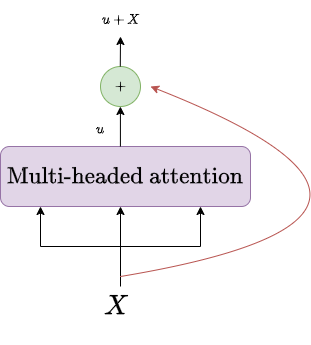
\includegraphics[width=0.3\linewidth]{images/transformers_images/residual_connection.png}
            \caption*{Our output contains direct information about the input. This hopefully improves training.}
        \end{figure}

        \begin{definition}
            In a \vocab{residual block}, the \gren{input} $x$ is added to the \purp{output} $F(x)$ of the block (in our case, multi-headed attention) .

            $$\text{output} = F(x) + x$$

            \begin{itemize}
                \item This is designed to reduce the risk of \orgg{vanishing gradient}, by directly exposing deeper layers to the input 
                \begin{itemize}
                    \item The long chain rule is what causes vanishing gradient: we've created a shorter chain rule.
                \end{itemize}
                
            \end{itemize}
        \end{definition}

            \note{If you ever hear someone refer to a "ResNet" or "Residual Network", this is a CNN that uses the same technique!}

    \phantom{}

    \subsection{Layer Normalization}

        Another topic from the NN chapter: \vocab{batch normalization}.\\

        \begin{definition}
            \textit{(Review from Neural Networks 2)}
            
            \vocab{Batch Normalization} is a process where we

            \begin{itemize}
                \item Standardize the pre-activation for each layer \orgg{across data points in the batch} using mean $\mu_i$ and standard deviation $\sigma_i$ (for the $\nth{i}$ dimension). 

                \begin{equation*}
                    \red{ \overline{Z}_{ij} } =  \frac{ \red{Z_{ij}}  -\blu{\mu_i}}{\sigma_i}
                \end{equation*}
                
                \item Choose the new mean and standard deviation for the pre-activation using $(n \times 1)$ vectors $G$ and $B$

                \begin{equation*}
                    \red{\widehat{Z}_{ik}} = \pur{G_i} * \red{\overline{Z}_{ij}} + \grn{B_i}
                \end{equation*}
            \end{itemize}
        \end{definition}

            \note{In short: we set the (mean, sd) to (0,1) and then scale it back up to $(G_i,B_i)$.}

        We would get the same kinds of benefits from \purp{normalization} in transformers as we did before in NNs. 
            \note{Stabilizing our training process, mostly.}

        But rather than normalizing across multiple \gren{data points} (batch), we'll normalize across the \purp{features} (layer) of a single token.\\

        \begin{kequation}
            Suppose we have a $(d \times 1)$ data point $z = \begin{bmatrix}
                z_1 & z_2 & \cdots & z_d
            \end{bmatrix}^T$. 
            
            \vocab{Layer normalization} computes the mean $\mu_z$ and standard deviation $\sigma_z$ across our \orgg{features} $z_i$

            $$\mu_z = \frac{1}{d} \sum_i z_i \qquad \qquad \sigma_z=\sqrt{\frac{1}{\mathrm{~d}} \sum_{i=1}^{\mathrm{d}}\left(z_i-\mu_z\right)^2} $$

            And then \purp{normalizes} them.

            $$z_{norm} = \frac{z - \mu_z}{\sigma_z}$$

            Finally, we scale them back up, to have mean $\beta$ and s.d. $\gamma$.

            $$\text{LayerNorm}(z; \gamma, \beta) = \gamma \Big( \frac{z - \mu_z}{\sigma_z} \Big) + \beta $$
        \end{kequation}

            \note{Layer normalization can be used on a single data point, while batch normalization requires many.}

        Now that we understand this process, we can apply this to our transformer model:

        \begin{itemize}
            \item After we get $u+x$ (creating the residual block), we use layernorm on each token separately:\\
        \end{itemize}

        \begin{concept}
            At the end of our \vocab{residual block}, we apply LayerNorm to each of our tokens separately

            \begin{itemize}
                \item We take our $(N \times d)$ object $u+X$ and normalize the features of each of our $N$ tokens (shape $(d \times 1)$) \purp{separately}.
            \end{itemize}

            $$\ex{u_{norm}}{i} = \text{LayerNorm}(\ex{u}{i}+ \ex{X}{i}, \gamma_1, \beta_1)$$
        \end{concept}

        \begin{figure}[H]
            \centering
            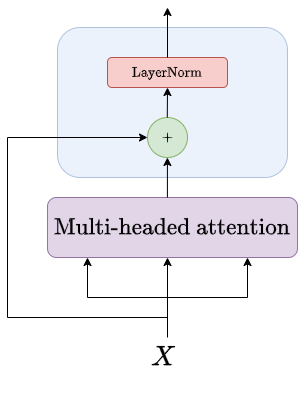
\includegraphics[width=0.3\linewidth]{images/transformers_images/multi_headed_attention_layernorm.png}
            \qquad \qquad
            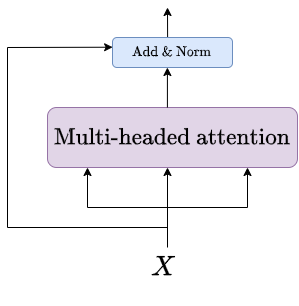
\includegraphics[width=0.3\linewidth]{images/transformers_images/multi_headed_attention_addnorm.png}
            \caption*{We append a LayerNorm layer. We'll follow the convention from the "\href{https://arxiv.org/pdf/1706.03762.pdf}{Attention is all you need}" paper and combine these into a single unit: "Add+Norm".}
        \end{figure}
        
        With this, our Residual Connection is complete.

    
    \pagebreak


    \subsection{Feed Forward}

        In our CNNs, after convolution, we would use a \orgg{fully-connected feed-forward network} to analyze the processed data.

        \begin{itemize}
            \item We'll follow the same sort of pattern here: the main difference being that we apply feed-forward after only \purp{one layer} of \gren{multi-headed attention}.\\
        \end{itemize}

        \begin{kequation}
            After we apply \orgg{Add \& Norm} to our Multi-headed attention, we run the output through a \vocab{feed-forward} layer, processing the data it receives.

            \begin{itemize}
                \item We use a linear layer $W_1$, a ReLU layer, and another linear layer $W_2$.
            \end{itemize}

            $$z = \grn{W_2^T} \;\text{\pur{ReLU}} \Big( \grn{W_1^T} u_{norm} \Big)$$

            
        \end{kequation}

        We can think of this as apply a hidden FC layer to our network, followed by another linear transform.

        \begin{figure}[H]
            \centering
            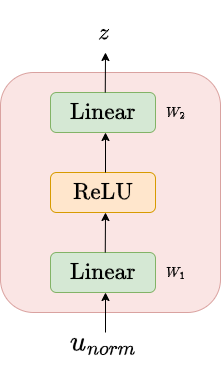
\includegraphics[width=0.15\linewidth]{images/transformers_images/feed_forward.png}
            \qquad \qquad
            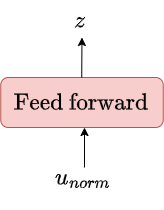
\includegraphics[width=0.15\linewidth]{images/transformers_images/feed_forward_compress.png}
            \caption*{Linear, ReLU, linear. Once again, following "\href{https://arxiv.org/pdf/1706.03762.pdf}{Attention is all you need}", we simply call this the "Feed forward" Layer.}
        \end{figure}

        We'll follow this up with another LayerNorm:
            \note{Meaning, we use another residual block.}\\

        \begin{concept}
            After our \vocab{feed-forward layer}, we apply \orgg{Add \& Norm} again.

            $$\ex{z_{norm}}{i} = \text{LayerNorm}(\ex{z}{i} + \ex{u_{norm}}{i}, \gamma_2, \beta_2)$$
        \end{concept}

        This is the final output of our \vocab{transformer block}.

        \begin{figure}[H]
            \centering
            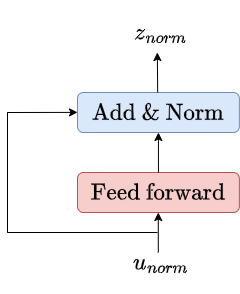
\includegraphics[width=0.2\linewidth]{images/transformers_images/feed_add_norm.png}
            \caption*{$z_{norm}$ is the final result of our transformer block.}
        \end{figure}


        

    \pagebreak  

    \subsection{Transformer Block}

        With this, we can assemble our transformer block, top to bottom:

        \begin{figure}[H]
            \centering
            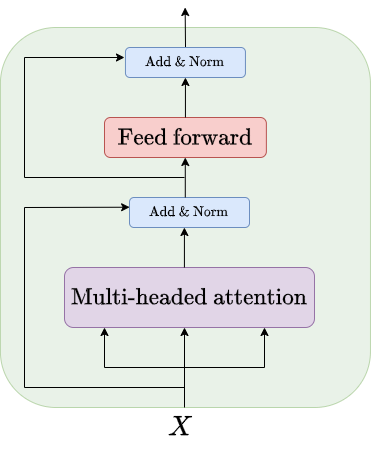
\includegraphics[width=0.35\linewidth]{images/transformers_images/transformer_block.png}
            \caption*{We have a transformer block!}
        \end{figure}

        \begin{definition}
            A \vocab{transformer block} is made up of several functions composed together:

            \begin{itemize}
                \item \purp{Multi-headed attention}
                
                    \begin{itemize}
                        \item Each head encodes the input text $X$ as keys $\ex{K}{h}$, a value ${Q}{h}$, and vectors $\ex{V}{h}$: one for each token.

                        \item Based on these, we compute \orgg{attention}.

                        \item Finally, we linearly combine information from across all $H$ heads.
                    \end{itemize}

                \item \gren{Add \& Norm}

                \item \redd{Feed-forward}

                    \begin{itemize}
                        \item We apply a fully-connected layer (linear+ ReLU), then another linear unit.
                    \end{itemize}

                \item \gren{Add \& Norm}
            \end{itemize}

            Both "Add \& Norm" layers accomplish the same thing: they create a \orgg{residual connection}.

            \begin{itemize}
                \item We add the input to the output, and then layer normalize.
            \end{itemize}
        \end{definition}

        \phantom{}

        \begin{concept}
            Each layer of our transformer block serves an important function:

            \begin{itemize}
                \item The \purp{multi-headed attention} layer explores connections between tokens, and provides information about the internal structure of our data.

                \item The \redd{feed-forward} layer processes our information nonlinearly (via ReLU).

                \item The \gren{add \& norm} layers create residual connections between the input/output of the preceding layer, improving our gradient-training process.
            \end{itemize}
        \end{concept}

        From here, we can design a transformer model by combining many of these transformer units in series.

        


    \pagebreak

    \subsection{Translation Task: training}

        We just have one more layer of complexity, before we finish. Let's consider a training example, for the task of translating from english to spanish.

        $$\text{I'm not hungry yet} \implies \text{Todavía no tengo hambre}$$

        Our transformer will start by predicting the \purp{first word} in the sentence: presumably "todavía".

            \begin{itemize}
                \item But not necessarily: if our model isn't \gren{well-trained} yet, it might predict some random word, like "espacio".
                    \note{It's also possible for us to have multiple valid translations, but we'll ignore that for now.}
            \end{itemize}

        Now, we want to predict the \textit{second word} in our output. But we just brought up an important problem:

        \begin{itemize}
            \item The best "second word" in our translation is \orgg{dependent} on the first word. We should factor that into our model, when predicting the second word.

            \item If our first word was wrong, then we're \purp{more likely} to use an incorrect second word!
        \end{itemize}

        The solution? Instead of using the first word we predicted, we use the \gren{correct} first word.

        \begin{itemize}
            \item Only one condition we need to remember: we need to \purp{mask} the rest of the "correct" output sentence, so our model can't use it to cheat.\\
        \end{itemize}

        \begin{concept}
            When \gren{training} our model to complete a language task, our model predicts each word (token) one-by-one, based on two pieces of data:

            \begin{itemize}
                \item The entire \gren{input prompt}
                \item The \purp{desired output} sequence for every token \orgg{before} the one we want to predict.
            \end{itemize}
        \end{concept}

        \miniex Suppose we're predicting the third word in our above sentence. We'll use the first two "correct" words as part of our model:
            \note{In this case, "tengo" is the word we want to predict.}

        $$\begin{bmatrix}
            \text{I'm not hungry yet} \\
            \text{Todavía no}
        \end{bmatrix}
        \implies
        \text{\red{tengo}}$$

        \begin{figure}[H]
            \centering
            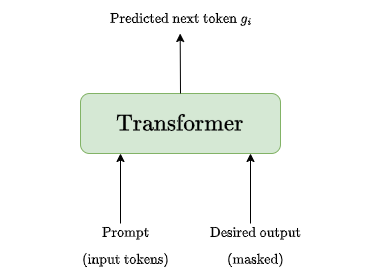
\includegraphics[width=0.35\linewidth]{images/transformers_images/text_prediction.png}
            \caption*{Our model is actually trained with \textit{two} inputs.}
        \end{figure}

        Something to take note of: we predict the $\nth{i}$ token based on the input, and the first $i-1$ \purp{desired inputs}.

        \begin{itemize}
            \item That means that, when predicting token $g_i$, we don't care what we predicted for the previous tokens!

            \item We don't need to finish predicting token $i$ to predict token $i+1$: we can do them at the same time!\\
        \end{itemize}

        \begin{concept}
            \vocab{Transformer Parallelization III}
        
            Predicting token $i$ is an independent calculation from predicting a second token $j$.

            \begin{itemize}
                \item That means we can predict every token in our sentence at the same time!
            \end{itemize}
        \end{concept}

        This is a \textit{huge} advantage in training transformers: it can essentially think about the entire sentence at the same time, massively speeding up training.\\

        \begin{clarification}
            We can't parallelize \vocab{token generation} when we're using our model \orgg{after} training:

            \begin{itemize}
                \item We can parallelize during training because we're using the \gren{desired output} for the previous $i-1$ tokens.

                \item When using our model for unseen data, we don't have "desired output": we have to use our \gren{actual output} for the previous tokens.
            \end{itemize}

            We have to \orgg{wait} for our model to predict the first $i-1$ tokens, before it predicts the $\nth{i}$ token.

            
        \end{clarification}


            
            

    \pagebreak

    \subsection{Encoder + Decoder Structure}

        Now, we have to structure our transformer model to be able to handle both the input and desired output.\\

        \begin{concept}
            There are three tasks we want our model to complete:

        \begin{itemize}
            \item \purp{Process} our input sequence,

            \item \purp{Process} our target sequence (desired output),

            \item \gren{Combine} the two sequences of information

            \item \orgg{Predict} the next character based on this data.
        \end{itemize}

        \end{concept}

        \begin{figure}[H]
            \centering
            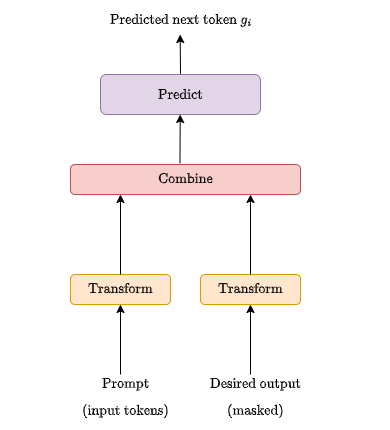
\includegraphics[width=0.45\linewidth]{images/transformers_images/encoder_decoder_proto.png}
            \caption*{We'll choose functions to handle each of these tasks.}
        \end{figure}

        \begin{itemize}
            \item We'll process our prompt using a complete transformer block. This unit is our \vocab{encoder}: we encode our prompt in a form that is more \gren{meaningful} to our computer.

            \item However, for our desired output, we'll only use \gren{attention}, learning about the internal structure of the output.
                \note{Why not add the feed-forward layer? We'll add it later: there's another component we want to add first (see below).}
            
                \begin{itemize}
                    \item We'll also use this unit to \purp{mask} our output (so our transformer can't "look ahead" at future tokens).
                \end{itemize}
        \end{itemize}

        \begin{figure}[H]
            \centering
            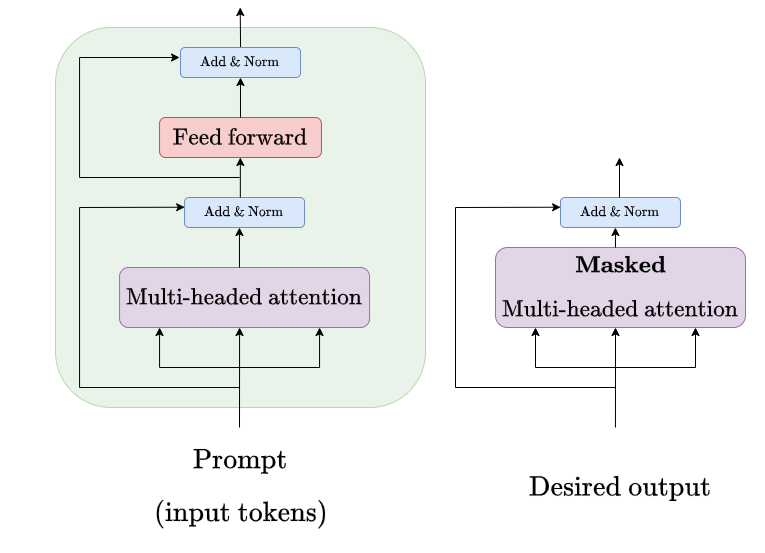
\includegraphics[width=0.6\linewidth]{images/transformers_images/attention_heads_encoder_decoder.png}
        \end{figure}

        We'll add the second feed-forward unit later. \purp{First}, we want to \gren{combine} information from our input, with the earlier tokens of our output.

        We accomplish this with another attention unit: this time, we'll use \vocab{cross-attention}.\\

        \begin{definition}
            In \vocab{cross-attention}, our \gren{queries} come from one sequence of text, while our \purp{keys/values} come from a \purp{different} sequence of text.

            \begin{itemize}
                \item As opposed to \orgg{self-attention}, where our keys/values/queries all come from the same sequence.
            \end{itemize}
        \end{definition}

        Our goal is to use the \gren{earlier} part of our \gren{output sentence} to determine which parts of our \orgg{input} we should \orgg{pay attention to} in our input sentence, when choosing the next token.
            \note{For example: if our output sentence already includes a word, it might be less likely we'll need to use that word again.}

        \begin{itemize}
            \item Our \gren{keys/values} represent the words we might want to \gren{pay attention to}.

            \item Our \purp{queries} help us decide \purp{what} to pay attention to.
                \note{We can use "attend" as a verb meaning "pay attention to": this is common when talking about transformers.
                
                \phantom{}
                
                For example, in this case, we're deciding "which input tokens to attend to".}
        \end{itemize}

        Thus, we'll use keys/values from our encoded input, and queries from our previous output tokens.\\

        \begin{concept}
            We integrate our \gren{input tokens} and our previous \purp{output tokens} using \vocab{cross-attention}: we apply attention, using

            \begin{itemize}
                \item Our encoded input as our \gren{keys and values}.

                \item Our attended output as our \purp{queries}.
            \end{itemize}

            This is our \vocab{encoder-decoder layer}.
        \end{concept}

        \begin{figure}[H]
            \centering
            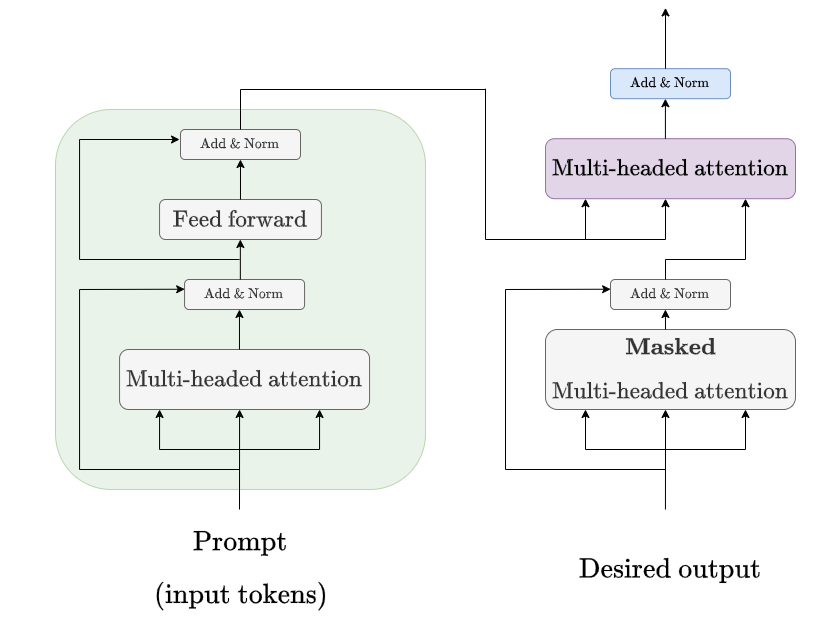
\includegraphics[width=0.65\linewidth]{images/transformers_images/cross_attention_decoder.png}
        \end{figure}

        Now that we've integrated information from both our input and output, we finally include our \orgg{feed-forward} unit: we'll process our integrated information.

        \begin{figure}[H]
            \centering
            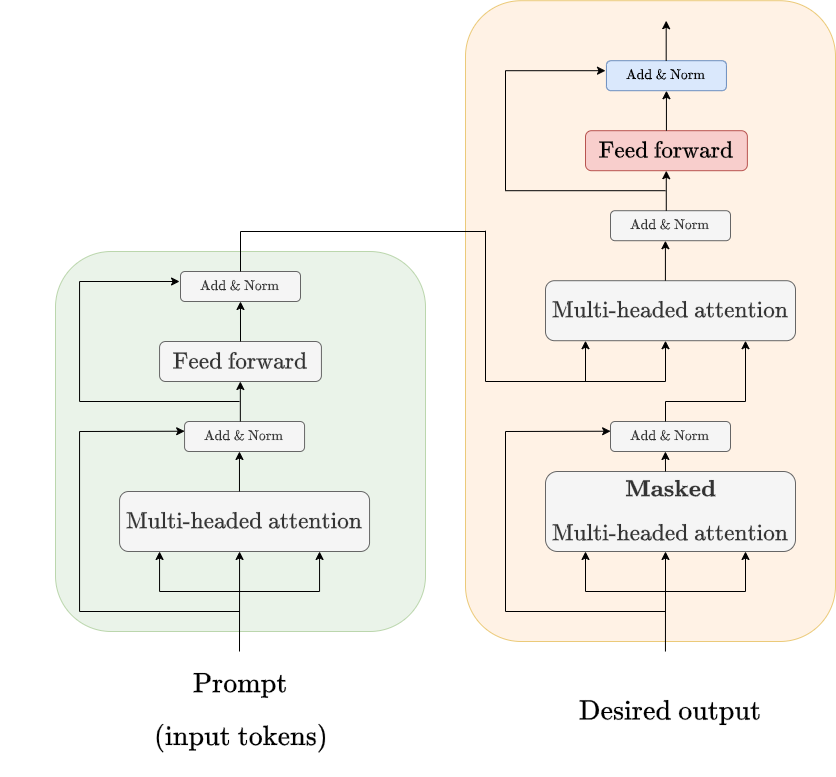
\includegraphics[width=0.65\linewidth]{images/transformers_images/decoder_feed_forward.png}
            \caption*{This unit on the right is called our \vocab{decoder}.}
        \end{figure}

        We've got a complete encoder/decoder setup:\\

        \begin{concept}
            We break our transformer into an "\gren{encoder}" and "\orgg{decoder}" unit:

            \begin{itemize}
                \item The encoder transforms our \gren{input} into a representation that contains more useful information: connections between tokens in the prompt, etc.

                \item The decoder transforms that encoding into a \orgg{output}/response: this decoder takes the information we've gathered, and applies it to our problem.
            \end{itemize}
        \end{concept}

        Consider the translation example:
        
        \begin{itemize}
            \item The encoder stores our English text in a form that hopefully represents the \purp{meaning}.

            \item The decoder "decodes" that representation into a form we can read, but in a \gren{different language}: Spanish, in our example.
        \end{itemize}

        In this analogy, we've created a special "code" that we write in English, and read in Spanish.

    \phantom{}

    \subsection{Predicting a token}

        Only one step left: using this decoded information, we need to \gren{choose} our token. This is the multi-class classification problem: we use the same protocol as we always do.

        \begin{itemize}
            \item We linearly transform our data: each token gets a "\purp{score}", based on how likely we think it is to be the correct one.

            \item We apply \orgg{softmax}, to turn these scores into probabilities. We get a probability for every possible token.
        \end{itemize}

        \begin{figure}[H]
            \centering
            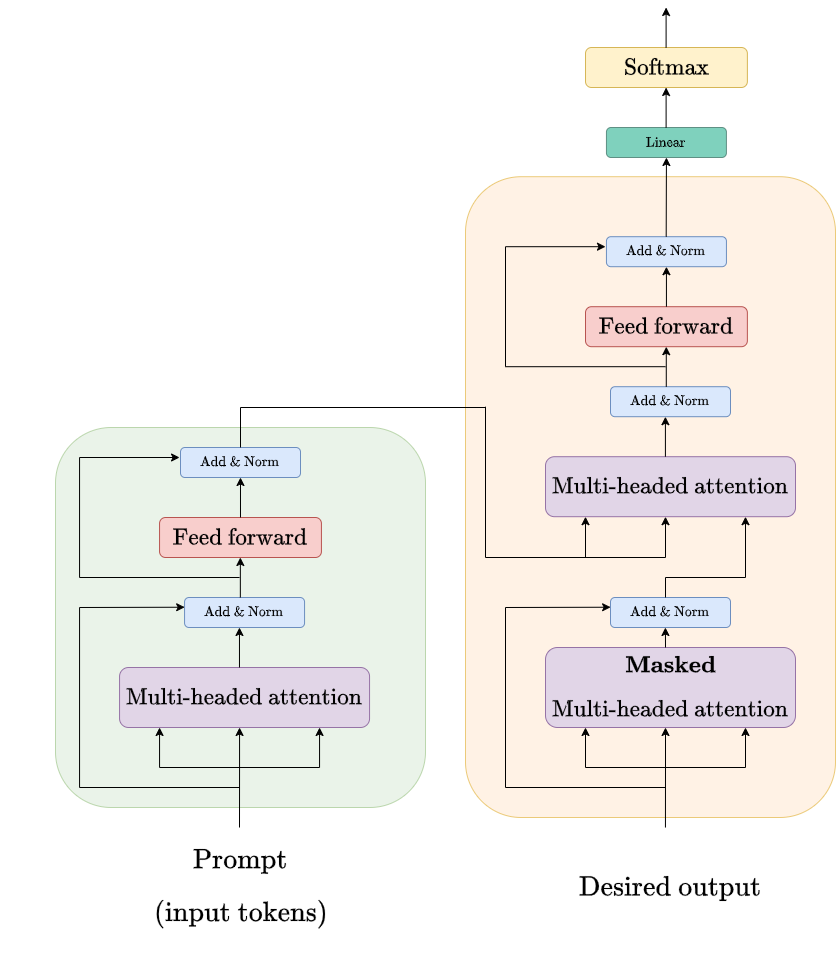
\includegraphics[width=0.65\linewidth]{images/transformers_images/transformer.png}
            \caption*{This is essentially a completed transformer.}
        \end{figure}

        This is the (now-famous) diagram from the "\href{https://arxiv.org/pdf/1706.03762.pdf}{Attention is all you need}" paper! 
            \note{We've excluded the initial embedding (turning words into vectors) and positional embedding (adding information about the position of each word in the sentence).
            
            \phantom{}
            
            We could include those for completeness, but that would just take up more space.}

        Only one detail still missing:

        \begin{itemize}
            \item Our decoder/encoder typically has \orgg{several copies} of the same unit in a row: for example, we might have 3 transformer blocks in a row for our encoder.
        \end{itemize}

        Notably, this is only one kind of transformer model: which architecture we use depends on the problem, cost constraints, etc.
            
        

        

        

    \pagebreak

    \subsection{Training Process}

        We typically train transformer models in two stages: pre-training and fine-tuning.\\

        \begin{definition}
            In \vocab{pre-training}, we expose our model to a very large dataset of human language, so it can learn \purp{patterns} in that language.

            \begin{itemize}
                \item We can use \orgg{unlabelled} data in this stage: thus, we have an unsupervised/self-supervised problem.
            \end{itemize}

            This stage of training is typically expensive.
        \end{definition}

        \phantom{}

        \begin{definition}
            In \vocab{fine-tuning}, we take our pre-trained model, and train it for a \purp{specific task}.

            \begin{itemize}
                \item We use \orgg{labelled} data in this stage.
            \end{itemize}

            It tends to be much faster and less expensive than pre-training.
        \end{definition}

    \phantom{}

    \subsection{Variations}

        We could make variations on this network:

        \begin{itemize}
            \item Use more/fewer decoder/encoder units.
            
            \item Use a different style of attention (rather than the dot product, we use some other similarity metric).

            \item Move LayerNorm to different parts of the network.
        \end{itemize}

\pagebreak

\section{Terms}

    \begin{itemize}
        \item Natural Language Processing (NLP)
        \item \textit{(Review)} Convolutional Neural Networks (CNNs)
        \item Locality
        \item Recurrent Neural Networks
        \item \textit{(Review)} Word Embedding
        \item Co-occurrence
        \item Context window
        \item Skipgram
        \item Word2vec
        \item Token
        \item Key Vector
        \item Query Vector
        \item Value Vector
        \item Attention Weights
        \item $d_k$
        \item Attention
        \item Self-attention
        \item Positional Encoding
        \item Masking
        \item Attention Head
        \item Projection Matrix
        \item Multi-headed attention
        \item Residual Block
        \item Residual Connection
        \item Layer Normalization
        \item Add \& Norm
        \item Feed-forward layer (transformers)
        \item Transformer Block
        \item Cross-attention
        \item Encoder (Transformers)
        \item Decoder (Transformers)
        \item Encoder-Decoder Layer
        \item Pre-training
        \item Fine-tuning
    \end{itemize}



        

        

    

    
        

